\chapter{ZCal-Calibrating radio interferometric data with machine learning}
\label{c3}
ZCal in full for "Zitha Calibration" is a new machine learning radio data calibration experiment whereby we make use of the telescope sensor data to find the relationship with the secondary calibrator solutions obtained with CASA. In Section \ref{Exp}, we further discuss the external parameters affection the observed radio interferometric data followed by a brief description of the KAT-7 telescope and how the sensor data  and calibration solutions are processed for training in  Section \ref{kat7}. In Section \ref{algo1} we define and describe the regression algorithms used for our experiment, and in Section \ref{TT} we describe the training and testing procedure of the algorithms leading to the output results of our experiment in Section \ref{sec3}. 
\section{External parameters affecting the data}
\label{Exp}
%%Each antenna in an array has a primary beam which is used for perfect resolution during an observation of a source. The resolution of each antenna is defined as =1.22 / D, where  ~ 21 cm is the  wavelength, D is the diameter of your dish and is the resolution angle. In an interferometric array of N antennas with baselines b, the resolution angle is defined as  =1.22  / d, where d is the maximum baseline in an array.   The beam of all the baselines is call a synthesised beam which is a multiplication of all the primary beams.

Astronomical observations done with interferometric radio
telescopes suffer from variable gain effects which can be
broadly classified as direction independent and direction dependent errors. The complex instrumental gains due to the electronic devices that follow the feed elements are directionally independent \citep{bhatnagar2008correcting}. Relative amplitude and phase gain for each antenna; phase and amplitude drifts in the electronics of each antenna; amplitude response as a function of elevation (gain curve) and tropospheric amplitude and phase effects.

As defined in Chapter 1, \textit{calibration} is the process of correcting for the signal corrupted by various mechanisms. Some of these mechanisms includes the external parameters like fluctuations in air-temperature, weather conditions on site and the antenna pointing errors \citep{taylor1999synthesis}. Antenna pointing error is the difference between the actual pointing position and the requested(to go) position. Though an array consist of more than one antenna each with tracking centre, during request ("POINT"),  they all must follow the same required position. However this is not always accurate due to misalignment of elevation axis, atmospheric refraction, gravitational deformation of the structure, differential heating of the structure and wind loading \citep{taylor1999synthesis}. Wind loading is an effect which degrade the pointing accuracy, thus the design of the telescope structure plays  role interms of wind loads \citep{smithdynamic}. Telescope with large dish structure are subjected to large wind loads. The wind speed and the geometric dimensions are the cause of the highly turbulent flows around the antenna. These are violent shifts in airflow on a surface and around the antenna \citep{upnere2012characterization}. Large errors can reduce the sensitivity of the telescope in \ref{sens}:
\begin{align}
\left[\frac{2kT_{sys}}{A_{eff}\sqrt{N(N-1)\tau \Delta \nu}}\right]
\label{sens},
\end{align}
 where ($N$ is the number of antennas in the array,  $A_{eff}$ is Aperture efficiency, $\tau$ is the integration time, $k=1.38\times 10^{-23}Jk^{-1}$ is the Boltzmann constant, $\Delta \nu$ is the bandwidth and $T_{sys}=\sum T_{i}$ an additive of noise contribution from different source such as atmosphere, ground, telescope surface and receivers) \citep{wilson2013tools}. This can also introduce distortion on sources that are resolved, i.e., objects that consist of a non point-like structure as opposed to the point sources in Figure \ref{pks1613} \citep{Calibration}. 



\section{KAT-7 Telescope}
\label{kat7}

\begin{figure}[H]
  \centering
    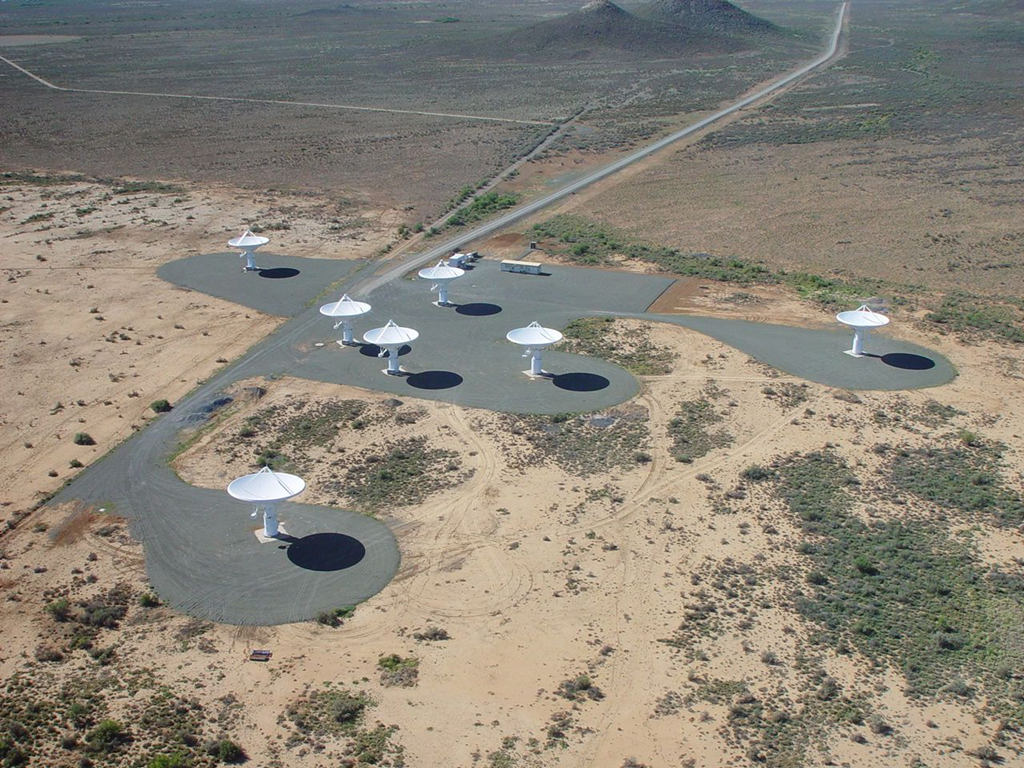
\includegraphics[width=0.6\textwidth]{images/K7.png}
    \caption{The seven-dish MeerKAT precursor array, KAT-7 \citep{carignan2013kat}}
  \label{images/kat7.png}
\end{figure}

The Karoo Array (KAT-7) is a seven dish interferometry which was built as an engineering prototype for technologies and techniques testing purposes in preparation for the 64-dish Karoo Array Telescope (MeerKAT). These instruments are located in the Northern Cape Karoo desert region and is operated remotely from CapeTown. The construction of  KAT-7 began in
2008 with the writing of the telescope requirements specification and was completed in 2010.  It was operated at an engineering mode until 2015  and became fully operational in 2016  \citep{foley2016engineering}. As seen in Table \ref{images/kat7.png}, KAT-7 antennas are extremely close together with baseline ranging between 26-185m \citep{carignan2013kat}. More parameter specifications are presented in the Tables \ref{DSpec},\ref{DSpec}:

\begin{table}[H]\centering
\begin{tabular}{l l }
\toprule
\textbf{Parameter} & \textbf{Value}\\
\midrule
Dish diameter&12m \\
Number of antennas& 7\\
Min baseline & 26m\\
Max baseline & 185m\\
Frequency range & 1200-1950MHz\\
Max instantaneous bandwidth &256MHz\\
Polarization   & Linear H $\&$ V\\
Systems temperature($T_{sys}$) & $<$35K across the entire frequency band\\
Aperture effeciency & 0.65\\
Location &  latitude 30.7148$^{\circ}$ S, longitude 21.388 $^{\circ}$ E\\
cryogenic temperature on receiver & 80K\\
Digital back end & Roach \\
Elevation & 1054m\\
\bottomrule
\end{tabular}
\caption{The 7 dish instrument each built with diameter 12m and linear polarization $H \& V$. The operational lower noise amplifier for each dish is $80K$  with system temperature $<35K$. The frequency range of this instrument is $1200-1950 \text{MHz}$ with bandwidth of $256\text{MHz}$ \citep{foley2016engineering}.}
\label{K7 spec}
\end{table}

%\begin{table}[H]\centering
%\begin{tabular}{l l l l}
%\toprule
%\textbf{Mode}& \textbf{Total BW(MHz)} & \textbf{Number of chan} & \textbf{Chan width(KHz)} \\
%\midrule
%c16n2M4k  &  1.5625	& 4096& 	0.381\\
%c16n7M4k & 6.25 & 	4096& 	1.526\\
%c16n25M4k& 	25&	4096& 	6.104\\
%c16n400M4k&  256& 	1024& 	390.625\\
%\bottomrule
%\end{tabular}
%\caption{The table is showing different correlator modes for observations. The correlator is based
%on the so-called 'FX, architecture, i.e (Fourier transform 'F' followed
%by Cross-correlation 'X'). The F  which channelise the incoming data streams
%into spectral components and the X does the multiplication and accumulation of each and every product pair \citep{foley2016engineering}.}
%\label{K7 modes}
%\end{table}

\begin{table}[H]\centering
\begin{tabular}{l l }
\toprule
\textbf{Parameter} & \textbf{Value}\\
\midrule
Pointing accuracy & 25 $^{\prime \prime}$ \\
Wind (Operational) & 36 km/h\\
Wind (Marginal Operation) km/h & 45 km/h\\
Wind (Drive to Stow) & 55 km/h\\
Wind (Survival) & 160 km/h\\
Azimuth Rotation slew speed &  2$^\circ$/s\\
Azimuth limits & -175$^{\circ}$, +285 $^{\circ}$\\
Elevation slew speed & 1$^{\circ}$/s\\
Elevation limits & 0$^{\circ}$, 90 $^{\circ}$\\
Feed/Cryo & Mass 75 kg\\
\bottomrule
\end{tabular}
\caption{The table is showing KAT-7 dish specification, each with pointing accuracy of 25 $^{\prime \prime}$. Each telescope is built with azimuth ranging from -175$^{\circ}$, +285 $^{\circ}$ and elevation drive ranging from 0$^{\circ}$, 90 $^{\circ}$. For protection of the dish from high wind conditions on site, the telescope is built to operate on 45 km/h windspeed and drive to protection mode at 55 km/h wind speed. \citep{foley2016engineering}.}
\label{DSpec}
\end{table}

\subsection{Sensor data}

During science observations, data indexed by time is continuously collected from instruments and  environment (atmospheric pressure, air temperature,  wind conditions, and relative humidity, wind direction, etc). Samples as a function of time are recorded from software and sensors attached to the telescopes with its adjoining instrumentation \citep{slabberICALEPCS2017}. Sampling strategies are set on sensors processed by the Control And Monitoring system (CAM), ranging from several updates per second to infrequent updates. The typical sample in KAT-7 CAM contains the following attributes: a sensor name, sample timestamp, value timestamp, status and a value as shown in the following example where red represents the sensor sample and green is the sensor sample description  \citep{slabber2015overview, slabber2015illustrate}. 

\definecolor{keywords}{RGB}{255,0,90}
\definecolor{comments}{RGB}{0,0,113}
\definecolor{red}{RGB}{160,0,0}
\definecolor{green}{RGB}{0,150,0}
 
\lstset{language=Python, 
        basicstyle=\ttfamily\small, 
        keywordstyle=\color{keywords},
        commentstyle=\color{comments},
        stringstyle=\color{red},
        showstringspaces=false,
        identifierstyle=\color{green}}

\begin{tcolorbox} 
\begin{lstlisting}

   {"name": "wx_station_wind_speed",
   "time": 1506430493.4778199196,
   "status": "nominal",
   "value_ts": 1506430493.4774999619,
   "value": 10.3}

   #SENSOR_NAME A normalised form of a sensor name.

   #SAMPLE_TS The UNIX timestamp of when the sample was
   #first processed by the CAM system.

   #VALUE_TS A UNIX timestamp when the acquisition
   #was performed. 

   #STATUS indicate the state of the sensor when
   #the sample was taken. Can have a value of UNKNOWN,
   #WARN, NOMINAL, FAILURE, INACTIVE, ERROR, UNREACHABLE. 
\end{lstlisting}
\end{tcolorbox}

All components are interfaced to the CAM system via the Karoo Array Telescope Communication Protocol (KATCP), i.e KATCP is responsible for internal communication between CAM components and other subsystems (Science data processing, Correlator Beamformer, etc) \citep{slabber2015overview}. A KATCP interface exposes requests and sensors. To access the sensor information for analysis, users from different subsystems  would  connect to the CAM webserver using Python client and subscribe to sensor data of interest. 

\subsection{Preparation of training data}\label{prep}

The objective of this study is to find correlations between
calibration solutions and sensor information on the telescope.
Therefore the main dataset for the study is the time based
sensor information of each antennae.
The process of data collection encompasses all of the steps required to obtain the desired data in a digital format. Methods of data collection include acquiring and archiving new observations, querying existing databases according to the science
problem at hand, and performing as necessary any cross-matching or data combining  \citep{ball2010data}.

%In this chapter we will look at modelling the behaviour patterns of individual antennas and calibration steps based on Karoo Array Telescope (KAT-7) \ref{images/kat7.png}.

In every observation, the collected data is stored by the data capturing system into the Hierarchical Data Format (HDF5), which is a set of file formats designed to store and organize large amounts of data. The HDF5 file is built into two concepts: meta data and observed visibilities. In meta data we find static information of the data set, including observer, dump rate and all the available subarrays and spectral windows in the data set selection criteria (antennas, channel frequencies, targets, scan information) and sensor data of interest as a function of time. The data observed by the radio telescope is in a form of complex numbers refereed to as visibilities as described in Chapter 1. Each source observed contains its own visibilities as a function of time along with sensor data  which keep record of the the telescope activity and behaviour as it observe.

In preparation of the training and testing dataset, we look at environmental sensors and instrumental sensors
recorded during observations with a flux calibrator and a phase calibrator source
PKS1613-586 in Figure \ref{pks1613}. This was the mostly used phase calibrator during Kat-7 commissioning phase. A series of observations for different tests with this calibrator \ref{pks1613} were taken between the period of December 2011 and November 2014. These tests includes Circinus X-1 monitoring at frequency $2022 - 1622.391 \text{MHz}$; OH maser monitoring at frequency $1666.481 - 1664.919 \text{MHz}$, $1666.381-1666.819\text{MHz}$,  $1666.281- 1664.719\text{MHz}$; Spectral dynamic range test at frequency $1669.125 - 1662.877 \text{MHz}$, $1678.500 - 1653.506 \text{MHz}$; Circinus X-1 H absorption at frequency $1425.125 - 1418.827 \text{MHz}$, $1424.125 - 1417.877 \text{MHz}$; Imaging new calibrators at frequency $2022 - 1622.391 \text{MHz}$. The chosen sensors of interested from each observation are listed in the following. 
\begin{enumerate}

\item Air temperature
\item Wind speed
\item Wind direction 
\item Air pressure 
\item Relative humidity 
\item Actual refraction elevation
\item Actual refraction azimuth
\item Actual scan elevation
\item Actual scan azimuth 
\item Actual pointing elevation
\item Actual pointing azimuth 
\end{enumerate}
The environmental sensors measures the environmental conditions on site via the weather station installed around the telescope; and the instrumental sensors (pointing) record the pointing azimuth and elevation activities of a telescope. These are the examples of how each environmental and instrumental sensor are represented per antenna X.

\definecolor{keywords}{RGB}{255,0,90}
\definecolor{comments}{RGB}{0,0,113}
\definecolor{red}{RGB}{160,0,0}
\definecolor{green}{RGB}{0,150,0}
 
\lstset{language=Python, 
        basicstyle=\ttfamily\small, 
        keywordstyle=\color{keywords},
        commentstyle=\color{comments},
        stringstyle=\color{red},
        showstringspaces=false,
        identifierstyle=\color{green}}
\begin{tcolorbox}
\begin{lstlisting}
   {"name": "anc_air_pressure",
   "time": 1506430493.4778199196,
   "status": "nominal",
   "value_ts": 1506430493.4774999619,
   "value": 981.65}
   
   {"name": "anc_gust_wind_speed",
   "time": 1506430493.4778199196,
   "status": "nominal",
   "value_ts": 1506430493.4774999619,
   "value": 3.96}

   {"name": "anc_air_temperature",
   "time": 1506430493.4778199196,
   "status": "nominal",
   "value_ts": 1506430493.4774999619,
   "value": 23.96}

   {"name": "anc_air_relative_humidity",
   "time": 1506430493.4778199196,
   "status": "nominal",
   "value_ts": 1506430493.4774999619,
   "value": 25.87}

   {"name": "anc_wind-direction",
   "time": 1506430493.4778199196,
   "status": "nominal",
   "value_ts": 1506430493.4774999619,
   "value": 46.61}
  
\end{lstlisting}
\end{tcolorbox}

\begin{tcolorbox}
\begin{lstlisting}
   {"name": "antX_pos.actual-pointm-elev",
   "time": 1506430493.4778199196,
   "status": "nominal",
   "value_ts": 1506430493.4774999619,
   "value": 89.97}
   
   {"name": "antX_pos.actual-pointm-azim",
   "time": 1506430493.4778199196,
   "status": "nominal",
   "value_ts": 1506430493.4774999619,
   "value": -78.81}
   
   {"name": "antX_pos.actual-refrac-elev",
   "time": 1506430493.4778199196,
   "status": "nominal",
   "value_ts": 1506430493.4774999619,
   "value": 89.80}
   
   {"name": "antX_pos.actual-refrac-azim",
   "time": 1506430493.4778199196,
   "status": "nominal",
   "value_ts": 1506430493.4774999619,
   "value": -70.15}
   
   {"name": "antX_pos.actual-scan-elev",
   "time": 1506430493.4778199196,
   "status": "nominal",
   "value_ts": 1506430493.4774999619,
   "value": 89.82}
   
   {"name": "antX_pos.actual-scan-azim",
   "time": 1506430493.4778199196,
   "status": "nominal",
   "value_ts": 1506430493.4774999619,
   "value": 78.94}
   
\end{lstlisting}
\end{tcolorbox}

We access this data from the HDF5 file using the KAT-7 data access library called katdal \citep{molenaar2017kern}. We select the sensor data of interest with time index during the telescope tracking of the flux calibrator and phase calibrator PKS1613-586. The following is a Python code example showing how the sensor time index is selected from the observations for a specific calibrator.

\begin{tcolorbox}
\begin{lstlisting}
#importing data access library
import katdal
import numpy
import time

#Opening the observation file 
hdf5=katdal.open('1329697773.h5')
#Selecting data of interest from the the observation file
hdf5.select(scans='track',
            targets=['PKS1934-63','PKS1613-586'],
            channels=slice(199,800)
            )   
#Obtaining sensor timestamps            
h5df5_timestamps=[]
temp_time = np.empty((len(h5.timestamps)))
for i in range(0,len(h5.timestamps)):
    temp_time[i]=(h5.timestamps[i])
    timeh5.append(T.ctime(temp_time[i]))      
       
#Selecting time during the scan of the calibrators
Time_Scan=[]
for scan in hdf5.scans() :
    #Taking average of start and endtime scan of calibrator source
    Average=((hdf5.timestamps[0]+
              hdf5.timestamps[len(hdf5.timestamps)-1])/2
             ) 
    Time_Scan.append(time.ctime(Average))
    
#obtaining time index of telescope sensors and scan time.
Time_index=numpy.where(np.in1d(numpy.unique(h5df5_timestamps),
                       Time_Scan))[0]
\end{lstlisting}
\end{tcolorbox}

 The Katdal library can manipulate the HDF5 observation file in many ways including file format conversion from HDF5 to measurement sets (ms). This option is useful for astronomers using CASA for data calibration and visualization \citep{foley2016engineering}. This conversion also provide an option whereby we flag all channels affected with known Radio Frequency Interference (RFI). Once the observation file was converted to ms format, hand flagging for unknown RFI was performed inside CASA using the task $\textit{flagdata}$ for $h$ and $v$ cross correlation products. After flagging the data and were satisfied, we then proceed to the calibration step. 
 
The systematic time-dependent complex gain errors denoted by $J_{ij}$ (where $i,j$ represent the baseline of two or more antennas) in the visibility data are almost always the dominant calibration effect, and a solution for them is necessary before proceeding with any other calibration \citep{ott2013casa}. In this thesis we only focus on the 1GC calibration with an interest of obtaining the complex gain calibration solutions for the phase calibrator PKS1613-586. In the process of 1GC, as explained in chapter 1, the complex gain calibration ($\textit{gaincal}$)  CASA task determines the time-based complex antenna gains solutions $G$ (amplitude \& phase) for each polarization h \& v and each spectral window, from the visibility data of the specified phase calibration source PKS1613-586 and store in calibration tables.
 
These solutions are calculated based on reference antenna 5 in our case, since it is an antenna that is approximately close to the center of the array and it was known to be particularly stable with no drop outs during KAT-7 commissioning \citep{ott2013casa}. The task $\textit{gaincal}$ in CASA factor $J_{i,j}$ into antenna-based components, so we do not see a set of values for each baseline, but rather only one for each antenna ($J_i$) \citep{CosmoAIMS}. 

Since our phase calibrator PKS1613-586 have an unknown flux density, the obtained values of the antenna based amplitude solutions differ from the correct ones by a factor depending only on the true source flux density by 

\begin{equation}
\frac{1 Jy}{(\text{true source flux density})^{0.5}},\;  \text{where 1Jy is the assumed flux density for \text{PKS1613-586}}.
\end{equation} 

We then used one of the following flux-density calibrators with known flux models: PKS1934-63, 3C147, 3C286 tied to the Perley-Taylor 99 to scale the correct gain amplitude of our phase calibrator in Figure \ref{pks1613} so that it match as well as possible the correctly-scaled amplitude solutions for the flux-density calibrators by running a CASA task $\textit{fluxscale}$ \citep{CosmoAIMS}. This process is called $\textit{Bootstrapping}$. After obtaining the final table with correct amplitude and phase complex gain solutions for the phase calibrator in Figure \ref{pks1613}, we then used the complex solutions matrix written on the "CPARAM" column to generate the training and testing calibration solution data per antenna $i$. An example of the complex gain amplitude and phase solutions is shown in Figure \ref{amp} and \ref{phase}. These solutions were obtained using the CASA task $gaincal$ described in Chapter 1. 

The following code is showing how the parameters were set in standard practice of 1GC as described in chapter 1 section \ref{caltech}.

\begin{tcolorbox}
\begin{lstlisting}
#Set flux for flux calibrator
default(setjy)
vis = msfile
field = flux_calibrator
fluxdensity  = -1
standard = 'Perley-Taylor 99'
setjy()

#Bandpass calibration
default(bandpass)
vis = msfile
caltable = bandpasstable
field = flux_calibrator
refant = reference_antenna
solnorm = True
combine = 'scan'
solint = 'inf'
bandtype = 'B'
minsnr = 5
interp = ['nearest']
bandpass()
\end{lstlisting}
\end{tcolorbox}
\begin{tcolorbox}
\begin{lstlisting}
#Calculating G solution for flux calibrator 
default(gaincal)
vis = msfile
caltable = gaintable
field = flux_calibrator
solint = 'inf'
refant = reference_antenna
gaintype = 'G'
calmode = 'ap'
solnorm = False
minsnr = 5
gaintable = [bandpasstable]
interp = ['nearest']
gaincal()
  
#G solution for gain calibrator
default(gaincal)
vis = msfile
caltable = gaintable
field = gain_calibrator
solint = 'inf'
refant = reference_antenna
gaintype = 'G'
calmode = 'ap'
append=True
solnorm = False
minsnr = 5
gaintable = [bandpasstable]
interp = ['nearest']
gaincal()   

#Scaling flux density for phase calibrator
default(fluxscale)
vis = msfile
caltable = gaintable
fluxtable = fluxtable
reference = flux_calibrator
transfer = gain_calibrator
fluxscale()
\end{lstlisting}
\end{tcolorbox}
A multi-frequency synthesis image deconvolution was carried using $\textit{CLEAN}$ CASA task with $256 \times 256$ and cell size of $30$ arc seconds. The image rms noise in Figure \ref{pks1613} was measured using the rms noise of the 0 iteration residual image.
\begin{tcolorbox}
\begin{lstlisting}
clean(vis='CircinusX-1.split.ms',imagename='PKS1613586.im',
     niter=10000,threshold='3.0mJy',
     psfmode='hogbom',
     interactive=False,
     imsize=512,
     cell='30arcsec',
     stokes='I',
     weighting='briggs',
     mode='mfs',
     usescratch=True)
\end{lstlisting}
\end{tcolorbox}
 \begin{figure}[H]
 \centering
    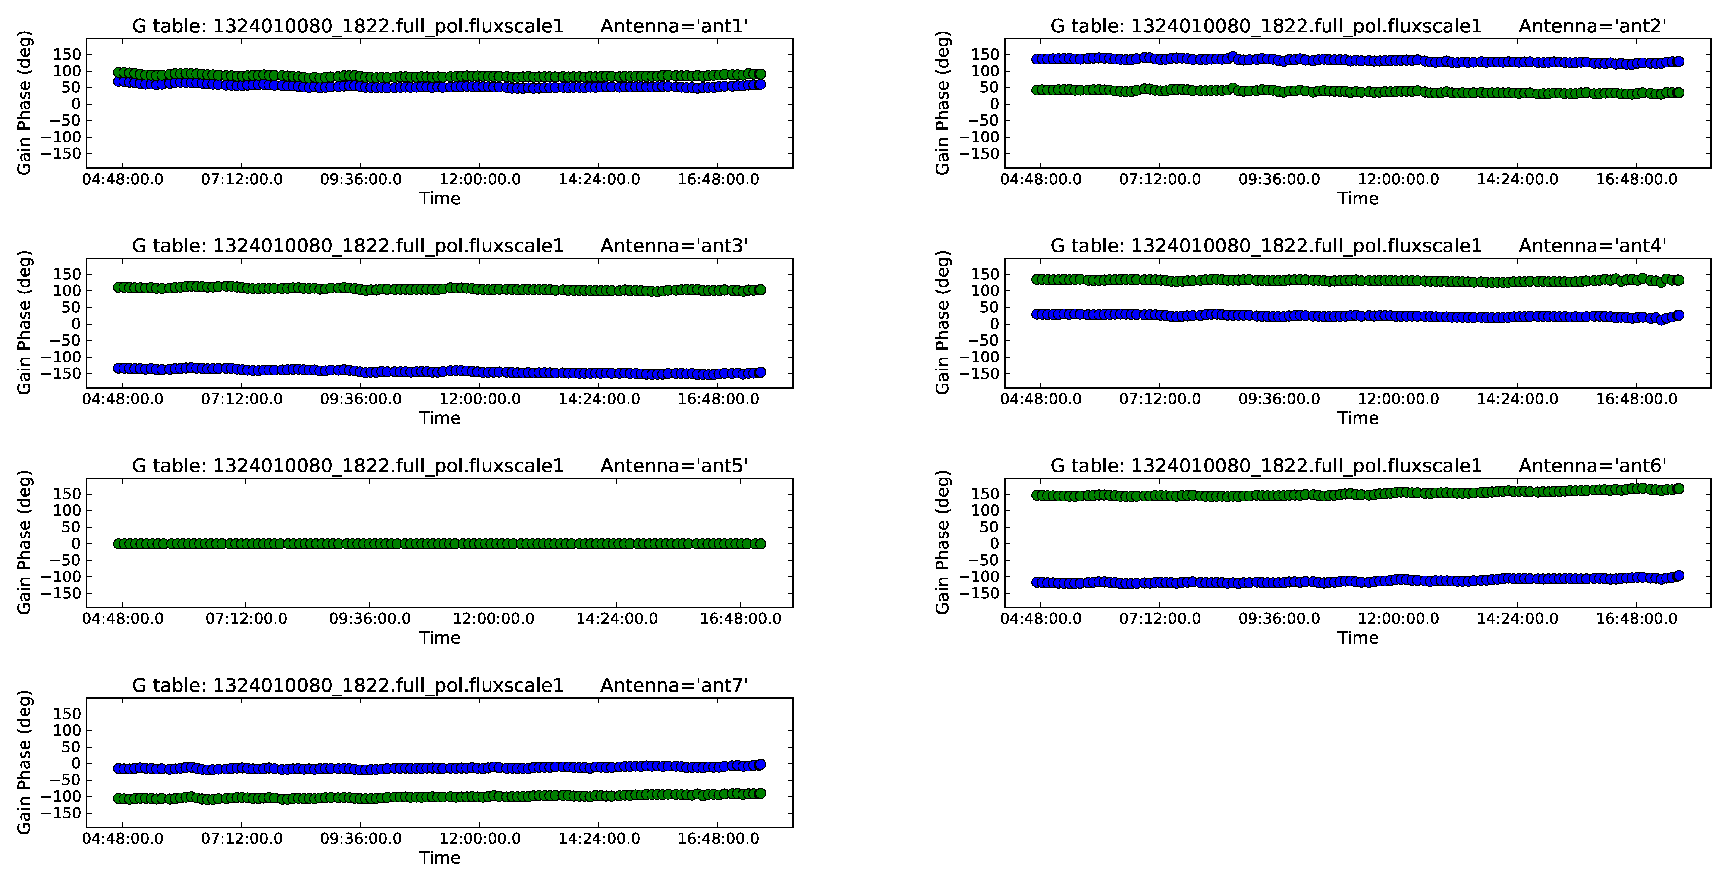
\includegraphics[ height=13cm, width=15.5cm]{images/phaseCasa.eps}
    \caption{Complex gain phase solutions for phase calibrator PKS1613-586 obtained from CASA per antenna i.Each colour represent different polarization where blue is H-polarization and green is v-polarization. Antenna 5 is showing zero phase since it is used as a reference antenna.}
  \label{phase}
\end{figure}

 \begin{figure}[H]
 \centering
    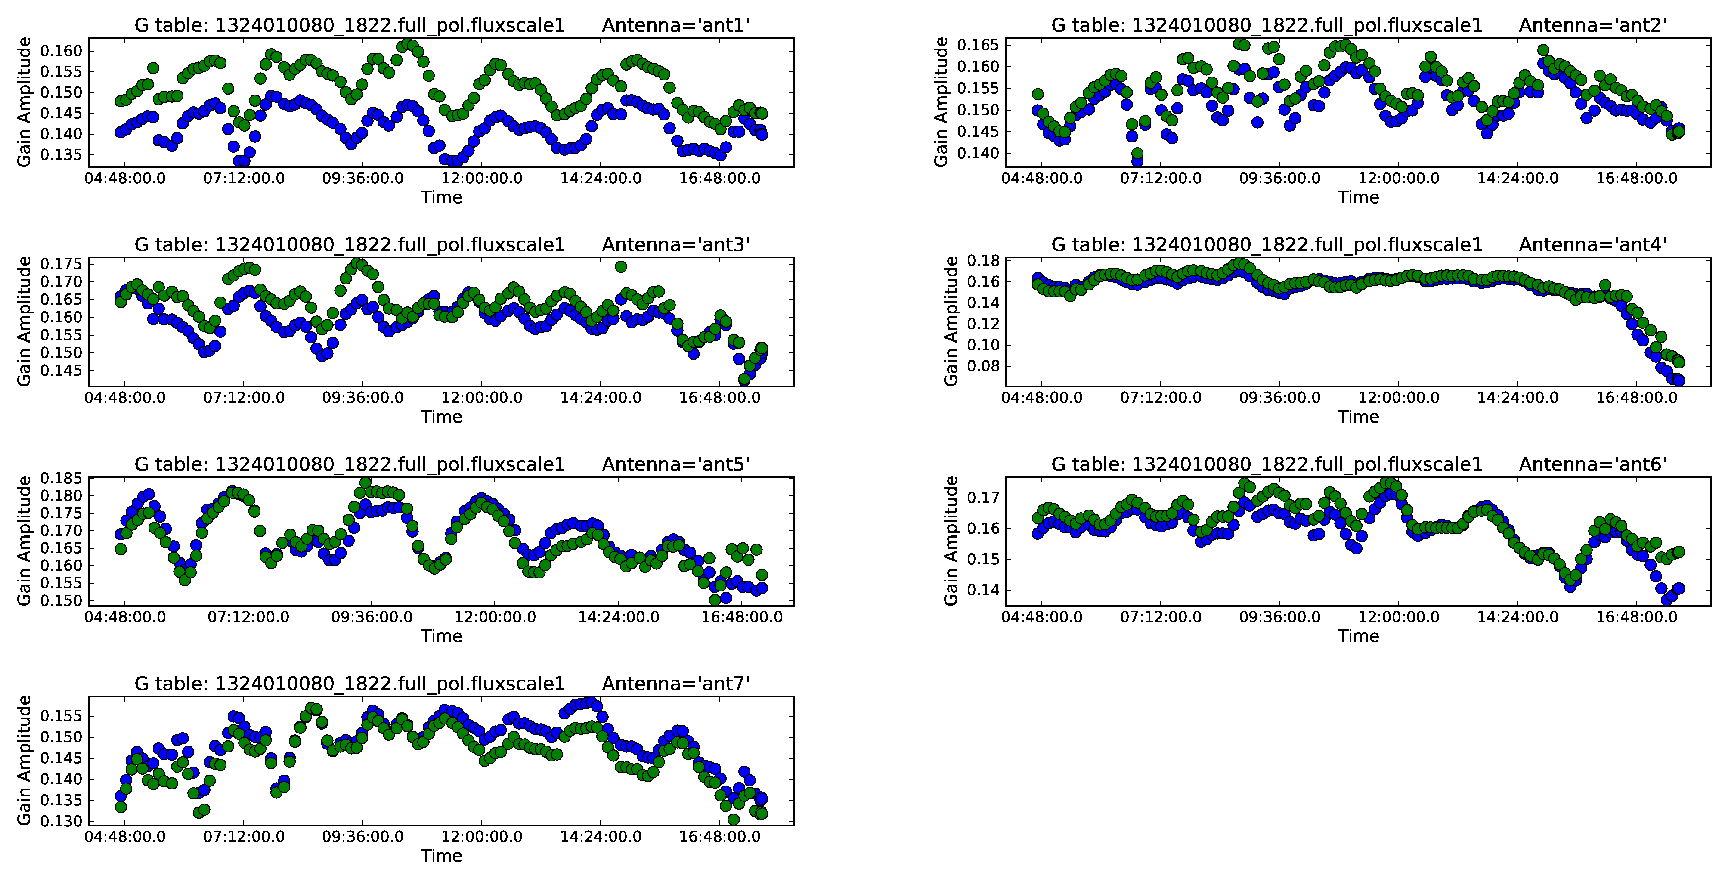
\includegraphics[ height=13cm, width=15.5cm]{images/CasaAmp.eps}
    \caption{Complex gain amplitude solutions for phase calibrator PKS1613-586 obtained from CASA per antenna $i$. Each colour represent different polarization where blue is H-polarization and green is v-polarization. }
  \label{amp}
\end{figure}
 
 \begin{figure}[H]
 \centering
    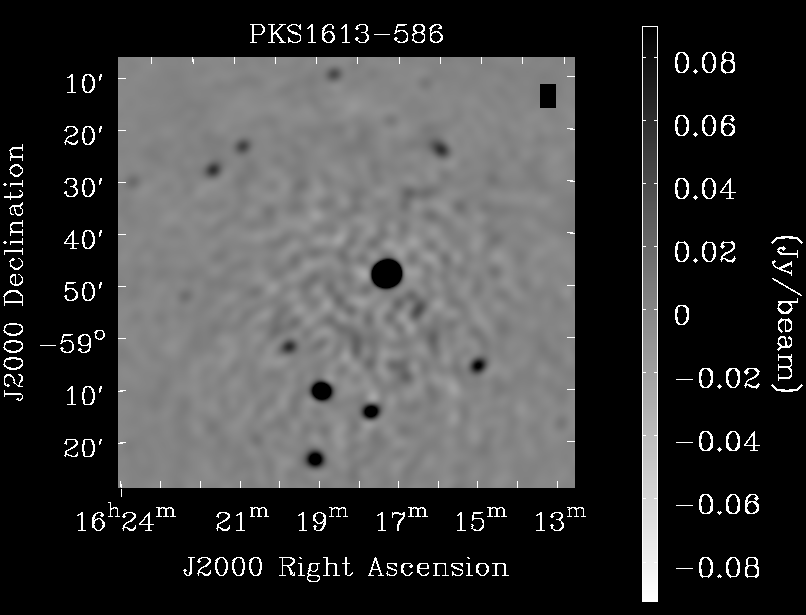
\includegraphics[ height=10.5cm, width=13cm]{images/162.png}
    \caption{An image of the phase calibrator PKS1613-586 located at RA, Dec (J2000): 16:17:17.88951, -58:48:07.8604. Its flux density in $Jy$ at $\text{frequency}=1.82688e^{+09} \text{Hz}$ is $4.59973 \pm 0.0146351$. This flux scaling was carried in CASA using a strong flux calibrator. The expected rms noise of this image was calculated to be $0.08Jy$ using $\textit{CLEAN}$ task in CASA.}
  \label{pks1613}
\end{figure}
\section{Regression algorithm} 
\label{algo1}
There are many different approaches employed in machine learning regression. These approaches learn the relationship between the input and output by fitting a model directly from the data. The fitting process involves the adjustment and optimization of hyper parameters to minimize the prediction error. This is usually done in an independent validation and testing dataset. In this study, we consider the tree based method approach: Decision tree, Random forest, Extremely randomized tree and the neighbourhood search approach: K-Nearest Neighbour to tackle our problem. Firstly, we formulate our regression estimation problem as follows. Suppose we have a feature matrix 
\begin{align*}
\textbf{X}_{t}=\begin{bmatrix}
    x_{11} & x_{12} & x_{13} & \dots  & x_{1n} \\
    x_{21} & x_{22} & x_{23} & \dots  & x_{2n} \\
    \vdots & \vdots & \vdots & \ddots & \vdots \\
    x_{d1} & x_{d2} & x_{d3} & \dots  & x_{dn}
\end{bmatrix}=(x_{i,j}) \in  \mathbb{R}^{d \times n}\;, i\in \left\{1,2,\dots, d\right\}, j \in \left\{1,2,\dots,n\right\}
\end{align*}
where each column represents a vector of length d containing unique features, 
\begin{align*}
\textbf{x}_j=\begin{bmatrix}
    x_{1,j}  \\
    x_{2,j} \\
    \vdots \\
    x_{d,j} 
\end{bmatrix},
\end{align*}
with each row a vector of length n, containing the n variable measurements for the ith observation, i.e 
\begin{align*}
\textbf{x}_i=\begin{bmatrix}
    x_{i,1}  \\
    x_{i,2} \\
    \vdots \\
    x_{i,n} 
\end{bmatrix},
\end{align*}

and we also have a matrix of complex target variables to learn and predict on,
\begin{align*}
\textbf{Y}_{t}=\begin{bmatrix}
    y_{11} & y_{12} & y_{13} & \dots  & y_{1m} \\
    x_{21} & y_{22} & y_{23} & \dots  & y_{2m} \\
    \vdots & \vdots & \vdots & \ddots & \vdots \\
    y_{d1} & y_{d2} & y_{d3} & \dots  & y_{dm}
\end{bmatrix}=(y_{k,l}) \in  \mathbb{C}^{d \times m},  k\in \left\{1,2,\dots, d\right\}, l \in \left\{1,2,\dots,m\right\}
\end{align*}
where each column represents a vector of length d, containing unique target variables as a function of time $t$
\begin{align*}
\textbf{y}_{l}=\begin{bmatrix}
    y_{1,l}  \\
    y_{2,l} \\
    \vdots \\
    y_{d,l} 
\end{bmatrix},
\end{align*} 
with each row a vector of length m, containing the m variable measurements for the kth observation, i.e 
\begin{align*}
\textbf{y}_k=\begin{bmatrix}
    y_{k,1}  \\
    y_{k,2} \\
    \vdots \\
    y_{k,m} 
\end{bmatrix},
\end{align*}
 
Our problem is to construct a learning machine $M:\textbf{X}_{t} \rightarrow \textbf{Y}_{t}$ which when given a validation set of sensor examples $\textbf{X}^*_{t}$, minimises some measure of discrepancy between its prediction $M(\textbf{X}^*_{t})\approx\widehat{\textbf{Y}}_{t}$ and the value of $\textbf{Y}_{t}$, where M represents the predictor. We measure the discrepancy using the commonly used statistical measures in regression \citep{borchani2015survey}. This includes the coefficient of determination, i.e

\begin{equation}
R^2\left[\textbf{Y}_{t},\widehat{\textbf{Y}}_{t}\right]=1-\frac{\sum_{k} \left[(\textbf{Y}_{t})_{k}-(\widehat{\textbf{Y}}_{t})_{k}\right]^2}{\sum_{k}\left[(\textbf{Y}_{t})_{k}-\overline{\textbf{Y}_{t}}\right]^2}, 0 \leq R^2 \leq 1,
\label{R2score}
\end{equation}
which simply measures how well the future observations are to be predicted by M, with the best score being 1 for the best performing predictor. 
where,  \begin{equation}
\overline{\textbf{Y}_{t}}=\frac{1}{d_{samples}} \sum_{k} (\textbf{Y}_{t})_{k},
\end{equation} 

is the mean value of $\textbf{Y}_{t}$ draw from d samples,  
 $\sum_{k}\left[(\textbf{Y}_{t})_{k}-\overline{\textbf{Y}_{t}}\right]^2$ is the total sum of squares which measures the total variance in the predictor and $\sum_{k} \left[(\textbf{Y}_{t})_{k}-(\widehat{\textbf{Y}}_{t})_{k}\right]^2$ the residual sum of squares (deviations predicted from actual values of data) which measures the discrepancy between $\textbf{Y}_{t}$ and $\widehat{\textbf{Y}}_{t}$ \citep{james2013introduction}.

The explained variance
\begin{equation}
V=\frac{\text{Var}\left[\textbf{Y}_{t}-\widehat{\textbf{Y}}_{t} \right]}{\text{Var}\left[\textbf{Y}_{t}\right]}, 0 \leq V \leq 1, 
\label{ExV}
\end{equation}  

measures the proportion to which the predictor accounts for the variation of of the observed data $\textbf{Y}_{t}$ \citep{bellinger2016fundamental}. The best possible score is considered to be 1. where 

\begin{align*}
\text{Var}\left[\textbf{Y}_{t}\right]&=\mathbb{E}\left[(\textbf{Y}_{t}-\mu)^2\right],\; \mu=\mathbb{E}\left[\textbf{Y}_{t}\right]\\
&=\mathbb{E}\left[\textbf{Y}_{t}^2-2\textbf{Y}_{t} \mu +\mu^2\right]\\
&=\mathbb{E}(\textbf{Y}_{t}^2)- 2\mathbb{E}(\textbf{Y}_{t} \mu) + \mu^2\\
&=\mathbb{E}(\textbf{Y}_{t}^2)-2 \mu^2 + \mu^2\\
&=\mathbb{E}(\textbf{Y}_{t}^2)-\mu^2,
\end{align*}
\citep{fortmann2012understanding}

and the mean squared error, mean absolute error, which measures the average of the squared and absolute of the errors between the the observed values $\textbf{Y}_{t}$ and the predicted $\widehat{\textbf{Y}}_{t}$. For accurate prediction of the predictor, the value of MSE and MAE should converge to zero \citep{james2013introduction}. 

\begin{align}
\text{MSE}\left(\textbf{Y}_{t},\widehat{\textbf{Y}}_{t} \right)=\frac{1}{d_{samples}} \sum_{k} (\textbf{Y}_{t}-\widehat{\textbf{Y}}_{t})^2_{k}
\label{MSE}
\end{align}

\begin{align}
\text{MAE}\left(\textbf{Y}_{t},\widehat{\textbf{Y}}_{t} \right)=\frac{1}{d_{samples}} \sum_{k} \left|\textbf{Y}_{t}-\widehat{\textbf{Y}}_{t}\right|_{k}
\label{MAE}
\end{align}.

The aim of this regression exercise is to predict multiple target variables $\widehat{\textbf{Y}}_{t}$  hence it is referred to as multi-output regression. The learned multi-target model will be used afterwards to simultaneously predict the values $\widehat{\textbf{Y}}_{t+1}$  of all target variables of the new incoming unlabeled instances $\textbf{X}_{t+1}$. It has been proven that multi-output regression methods yield to a better predictive performance and also provide to means to effectively
model the multi-output datasets by considering not only the underlying relationships
between the features and the corresponding targets but also the relationships between
the targets, thereby producing simpler models with a better computational efficiency. From \citep{borchani2015survey}, several applications of multi-output regression are discussed including simultaneous estimation of different biophysical parameters from remote sensing images, channel estimation through the prediction of several received signals, etc. Further discussions, it is mentioned that these applications give rise to challenges such as missing data, i.e, when some features or target variables are not observed.

\subsection{Decision tree}
\label{Dt}
Decision trees algorithms are popular methods for machine learning tasks such as classification and regression. These algorithms are easy to handle categorical features, interpret, extend to the multi-output for regression settings and multiclass for classification setting. They can handle datasets that may have errors, missing values and are able to capture non-linearities and feature interactions \citep{DT}, hence they are widely used. One of the biggest advantages of using decision trees is the ease in which we can see what features or variables contribute to the classification or regression and their relative importance based on their location in the tree.

For a response variable which
has classes, the tree algorithm (classification) organizes the dataset into groups by the response based on the similarities of the data, and when the response variable is numeric or continuous, the tree algorithm (regression) uses the data to predict the outcome by fitting the regression model in each of the independent variables \citep{morgan2014classification}.

Decision trees are simple but powerful form of multi-variable analysis, they  perform a recursive binary partitioning of the feature space. The term binary refers to the fact that the parent node  will always be split into exactly two child nodes \citep{moisen2008classification}. The term recursive is used to indicate that each child node will, in turn, become a parent node, unless it is a terminal node as illustrated in Figure \ref{images/DecisionTree} where the split occurs at the decision node.  

Decision trees are build by growing a tree upside down starting from the root node. The data sample passes down the tree through a series of splits, or nodes, at which a decision is made as to which direction to proceed either left or right sub-tree based a sequence of questions about the features \citep{musicant2007supervised}. The next split or decision made depends on the answers to previous questions. Eventually, a terminal node is reached and the prediction is made.  

 \begin{figure}[H]
  \centering
    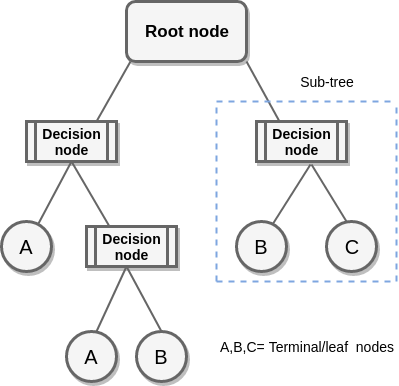
\includegraphics[width=0.6\textwidth]{images/DC.png}
    \caption{An illustration of decision tree where a recursive partition is shown from root node where there is an entire data sample to the internal nodes (decision nodes) where splitting occur to form child nodes which are either decision nodes or terminal nodes. Terminal node implies that after this split, further splitting of the samples does not provide relevant information in predicting the response variable \citep{moisen2008classification}. }
  \label{images/DecisionTree}
\end{figure}

The binary recursive partitioning, applies to the fitting of both classification and regression trees, where in both cases the variable and the location of the split are
chosen to minimize the impurity of the node at that point. However the selection criteria of splitting each node are different for these two methods. In our case for regression scenario, the splitting rules used to minimize the impurity of each node $c$ with number of samples $N_{c}$ and training data $\textbf{X}_{c}$ is the mean square error \citep{morgan2014classification}.
\begin{align}
\text{MSE}\left(\textbf{X}_{c}\right)=\frac{1}{N_{c}} \sum_{i\in N_{c}} (\textbf{Y}_{i}-\mu_{c})^2,
\end{align}  
which minimizes the mean of the sum of the square of the differences between the target value $\textbf{Y}_{i}$ and the estimated value $\mu_{c}$ \citep{moisen2008classification},
 
where  $$\mu_{c}=\frac{1}{N_{c}} \sum_{i\in N_{c}} \textbf{Y}_{i}$$ is the sample mean of the response variable which represents the  assigned prediction in each terminal node.

The mean absolute error  
\begin{align}
\text{MAE}\left(\textbf{X}_{c} \right)=\frac{1}{N_{c}} \sum_{i\in N_{c}} \left|\textbf{Y}_{i}-\mu_{c}\right|, 
\end{align}
 which minimizes the mean of the sum of the absolute differences between the target $\textbf{Y}_{i}$ and the estimated value  $\mu_{c}$ \citep{moisen2008classification}. These methods does not only measure the impurity in each node, but they are also used to measure the accuracy of the predictor as in equation \ref{MSE} and \ref{MAE}. Another commonly used strategy or measure in classification problems which also applies in regression problem for selecting the best split from a set of possible split is to maximize the information gain at each tree node. i.e, the split chosen at each decision node is chosen from the the set $\text{argmax} IG(\textbf{X}_{c},s)$ where $IG(\textbf{X}_{c},s)$ is the information gain when a split $s$ is applied to sample data $\textbf{X}_c$. This is the difference between the parent node (decision node) impurity and the weighted sum of the child nodes in equation \ref{IG}. 
 
 \begin{align}
 IG(\textbf{X}_c,s)&= \text{Impurity}(\textbf{X}_c)-\frac{N_{c(left)}}{N_c}\times \text{Impurity}(\textbf{X}_{c(left)})- \frac{N_{c(right)}}{N_c}\times \text{Impurity} (\textbf{X}_{c(right)}), \label{IG}
 \end{align}
 where $s$ is a split partitioning the training sample $\textbf{X}_c$ of size $N_c$ into two datasets $\textbf{X}_{c(left)}$ and $\textbf{X}_{c(left)}$ each of size $N_{c(left)}$ and $N_{c(right)}$.
If the impurity measure is the mean squared error, we therefore define the information gain by
 \begin{align}
 IG(\textbf{X}_c,s)&= \text{Impurity}(\textbf{X}_c)-\frac{N_{c(left)}}{N_c}\times \text{MSE}_{(left)}- \frac{N_{c(right)}}{N_c}\times \text{MSE}_{(right)}.
  \end{align}
If the impurity measure is the mean absolute error, the information gain is defined by   
 \begin{align}
 IG(\textbf{X}_c,s)&= \text{Impurity}(\textbf{X}_c)-\frac{N_{c(left)}}{N_c}\times \text{MAE}_{(left)}- \frac{N_{c(right)}}{N_c}\times \text{MAE}_{(right)} 
 \end{align}
 
For multi-output decision trees which predict multiple continuous target attributes at once, the advantage over building a separate
regression tree for each target is that the built tree is usually much smaller than the total size of the individual single-target trees for all variables, second, they identifies the dependencies between the different target variables in a better manner.

The building of the multi-output decision trees follows  the same steps as the standard decision tree in Figure \ref{images/DecisionTree}. Starting with all instances in the root node, then iteratively finding the optimal split and partitioning the nodes accordingly until a terminal node is reached given a certain stopping criterion. The only difference  is the redefinition of the impurity measures in equation \ref{MSE} and \ref{MAE} of a node as the sum of the squared error  over multi-target response. 
\begin{align}
\sum_{k\in d}\frac{1}{N}\left[\sum_{l \in N }\left(\textbf{y}_{k}^{(l)}-\mu^{(l)} \right)^2\right],
\end{align}
where $\mu^{(l)}$ denotes the predicted output for the instance $l$ in each node. Each split is selected to minimize the sum of the squared error such that each terminal leaf of the tree can be characterized by the multi-variate mean
of its instances and its defining feature values.

\subsection{Random forest}
While classification and regression trees are powerful methods in and of themselves, much work has been done in machine learning to improve the predictive ability of these tools by combining separate tree models into what is often called ensemble.

Random Forests is a combination (ensemble) of decision tree predictors such that each tree depends on the values of a random vector sampled independently and with the same distribution for all trees in the forest as shown in Figure \ref{random tree} \citep{breiman2001random}. This algorithm  was introduced by \citep{ho1995random} after having noticed that decision trees were limited in their accuracy due to their inability to grow in arbitrary complexity. This method was not only more accurate, but it was less susceptible to overfitting.

 \begin{figure}[H]
  \centering
    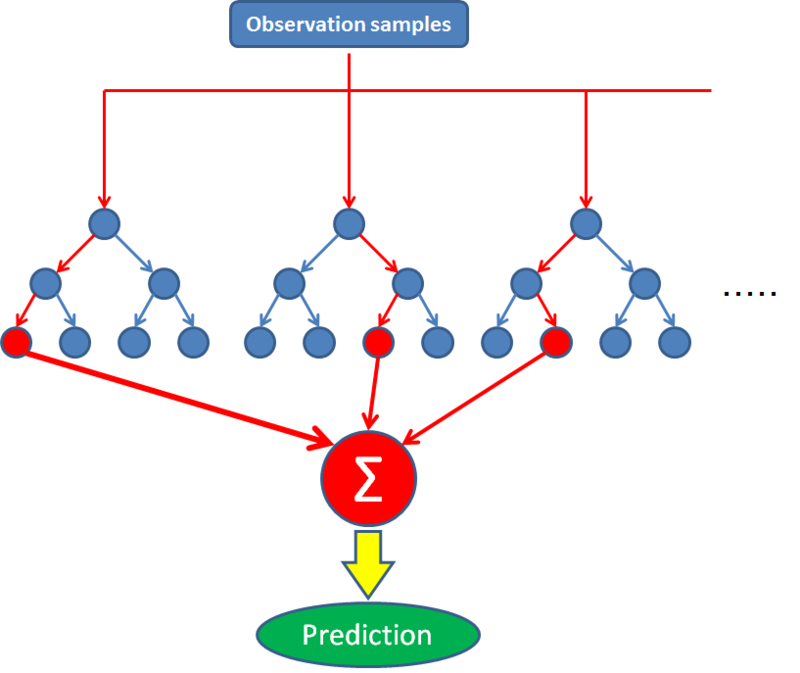
\includegraphics[width=0.6\textwidth]{images/RandomForestTree.png}
    \caption{Random forest regression. [image by Data scientist TJO in Tokyo]}
  \label{random tree}
\end{figure}

During the construction of a component decision tree, at each step
of split selection, random forest first randomly selects a subset of features, and then carries out the conventional split selection procedure within the selected
feature subset. Note that the randomness is only introduced into
the feature selection process, not into the choice of split points on the selected feature. Random forest is an extension of bootstrap aggregating (Bagging) where the major difference difference with bagging is the incorporation of randomized feature selection \citep{zhou2012ensemble}. The operational procedure of bagging is as follows: 

\begin{itemize}
\item Given a a set $\textbf{X}$ of size $\textit{N}$.
\item Generate $\textit{m}$ subsets in vector $\Theta$  of length $\textit{n}$ by randomly selecting data from the set $\textbf{X}$ with replacement \citep{breiman2001random}. 
\item Run $\textit{k}$ number of trees for each of the $\textit{m}$ sets of $\Theta$ to train the data.
\item This will generate $\Theta_{\textit{m}}$ sets of trained data.
\item For the remaining $\textit{n}$ sample, trained trees from the previous two steps can be fitted onto the remaining
data set of $\textbf{X}_{\textit{n}}$ to estimate the features of the data.
\end{itemize}

The parameter $\textit{k}$ controls the incorporation of randomness and this results on an increase in the bias. When $\textit{k}$ equals the total number of features, the constructed decision tree is identical to the traditional deterministic decision tree, when $\textit{k}$ = 1, a feature will be selected randomly. The suggested value of $\textit{k}$ is the logarithm of the number of features \citep{breiman2001random}.

The predictions of the trees that are constructed by the random forest are aggregated (majority voting for classification or averaging for regression) to produce the final output prediction. Suppose the underlying true function we try to learn is $f(\textbf{x})$, and $\textbf{x}$ is sampled according to a distribution p($\textbf{x}$). The output of each decision tree learner can be written as the the true value plus an error item, i.e.,
\begin{align}
h_{i}(\textbf{x})= f(\textbf{x}) + \epsilon_{i} (\textbf{x}), i = 1, \dots,T.
\label{hx}
\end{align}
such that we have the averaging and, 
\begin{align}
H(\textbf{x})= \frac{1}{T}\sum_{i=1}^{T} h_{i}(\textbf{x}). 
\label{averageRF}
\end{align}
\citep{zhou2012ensemble}

Recall in Section \ref{Dt}, that the prediction of  each tree is the sample mean, then from equation \ref{hx} we thus have the mean squared error of the output prediction $h_i$ as 
\begin{align}
\int (f(\textbf{x})-h_{i}(\textbf{x}))p(\textbf{x})^2d\textbf{x} = \int \epsilon_{i} (\textbf{x})^2 p(\textbf{x})d\textbf{x}
\end{align}
Similarly we can derive the mean square error of the combine decision tree learner (i.e, the ensemble) is 

\begin{align}
\int \left(f(\textbf{x}) - \frac{1}{T}\sum_{i=1}^{T} h_{i}(\textbf{x}) \right)^2  p(\textbf{x})d\textbf{x} = \int \left( \frac{1}{T}\sum_{i=1}^{T} \epsilon_{i}(\textbf{x})\right)p(\textbf{x})d\textbf{x}
\end{align} 


The two main parameters of RF are the number of trees grown and the number of predictors randomly tried at each split. What you call depth is sometimes found as the maximum node size, and controls the size of the trees that are grown. In the original implementation of RF, trees are grown to the maximum potential extent so that they reach the lowest possible bias. Then, variance is reduced by growing many trees and averaging them. The main reason being that in RF, you can only decrease error by reducing the variance, so the bias needs to be as low as possible in the first place. Therefore, in most cases, you don't really need to adjust this parameter (depth or max nodesize). Just make sure the default value allows the trees to grow as deep as possible.

\subsection{K-nearest neighbour}

The K-nearest neighbors algorithm is a well known non-parametric algorithm commonly used for regression and classification problems. This algorithm does not make any assumptions about the distribution of the data being evaluated, i.e, the model structure is determined from the data. The learning technique used in in K-nearest neigbors is known as the instance Based Learning. This technique is based on the memorization of the training dataset and the number of parameters is unbounded and grows with the size of the data. 

The intuition underlying nearest neighbor regression is quite straightforward,
the output predictions are obtained by looking into the memorized examples where the cost of the learning process is 0. The cost is in the computation of the prediction, with the prediction output being the continuous average values (or median) of the values of its K nearest neighbors. The commonly used measure in K-nearest neighbors is the distance functions , i.e, consider $\mathcal{M}$ the m-dimensional Euclidean space $\mathbb{R}^m$  , a training data set $\textbf{X}=\{\textbf{x}_1,\dots, \textbf{x}_n\} \subset \mathcal{M}$, a query point $q\in \mathcal{M}$, and a distance metric $d:\mathcal{M}^2 \rightarrow \mathbb{R}$. The K-nearest neighbor search is the task of finding  the K closest (w.r.t $d$ ) points to $q$ from the data set $\textbf{X}$, i.e, we find a set $\textbf{A} \subset \textbf{X}$ for which it holds  that $|\textbf{A}|= K$ and  $d(q,\textbf{x})\leq d(q,\textbf{y})$ $\forall$ $\textbf{x}\in \textbf{A}, \textbf{y}\in \textbf{X} \;\text{or}\; \textbf{A}$ \citep{hyvonen2015fast}. 

The distance function is defined as 
\begin{align}
d(\textbf{x},\textbf{y})= \sum_{i=1}^m \left(|x_i -y_i|^m\right)^{\frac{1}{m}}
\end{align}
known as Minkowski distance. For special case where $m=1$ the distance function is a Manhantan distance also know as the L-1 norm
\begin{align}
d(\textbf{x},\textbf{y})= \sum_{i=1}^m|x_i -y_i|,
\end{align}
and if $m=2$, the distance function is a Euclidean distance, also know as the L-2 norm and, 
\begin{align}
d(\textbf{x},\textbf{y})= \sqrt{\sum_{i=1}^m \left(x_i -y_i \right)^2}
\end{align}
\citep{cunningham2007k}

\begin{figure}[H]
  \centering
    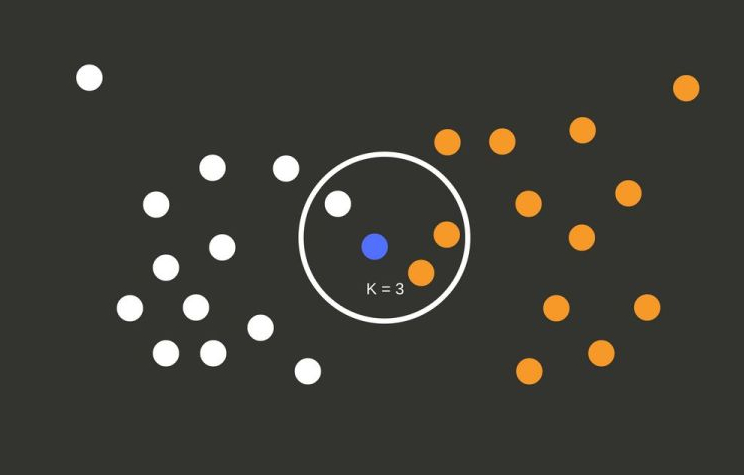
\includegraphics[width=0.5\textwidth]{images/Kn.jpg}
    \caption{Example of K-nearest neighbor. We have two different target classes white and orange circles. We have total 26 training samples. Now we would like to predict the target class for the blue circle. Considering k value as three, we need to calculate the similarity distance using similarity measures like Euclidean distance \citep{K-NNALGORITHM}.}
  \label{kn}
\end{figure}

\subsection{Extremely randomized tree}

Extremely randomized tree is another tree-based ensemble method for supervised classification and regression problems. It builds an ensemble of decision trees according to the classical top-down procedure in Figure \ref{random tree}. Its differences with other tree-based ensemble methods (random forest) are that the nodes are being split by choosing a threshold (cut-point) at random, and that it uses the whole training dataset rather than the bootstrap replica to grow the trees.  

As in random forest, the predictions of the trees are also aggregated to yield the final prediction, by majority vote in classification problems and arithmetic average in regression problems as shown in equation \ref{averageRF}. The explicit randomization of the cut-point and ensemble averaging reduces the variance even more, i.e $\text{Error}=\text{bias} - \text{variance}$ \citep{geurts2006extremely}. 
\section{Training and Testing}
\label{TT}
The process of training and testing involves feeding a learning algorithm with training data (seen data) to learn from by finding suitable parameters and evaluate its performance using testing data (unseen) as illustrated in Figure \ref{overview}. A fundamental assumption of machine learning is that the training data is representative of the distribution from which future data  will be chosen \citep{witten2016data}. Each instance in the training set contains "target value" and several "attributes" (namely features). 

\begin{figure}[H]
  \centering
    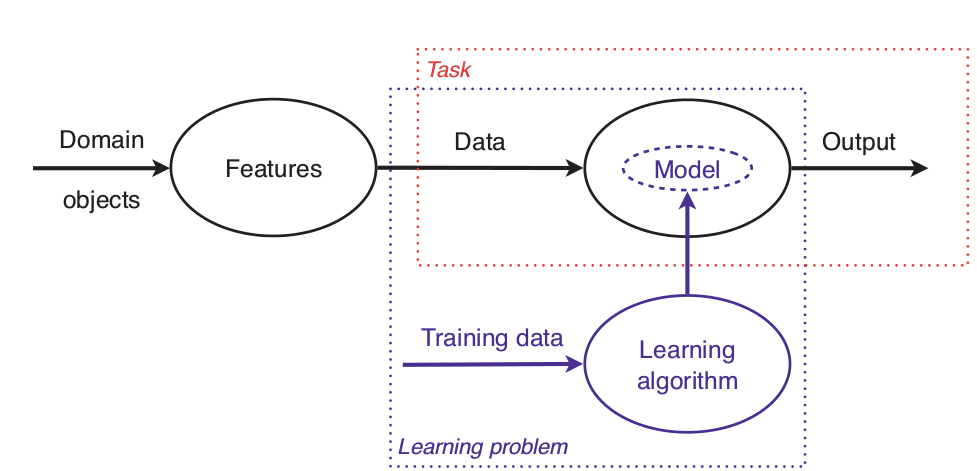
\includegraphics[width=0.7\textwidth]{images/MLSampler.png}
    \caption{An overview of a machine learning model training \citep{flach2012machine}.}
  \label{overview}
\end{figure}

Referring Section \ref{prep}, the challenges and the difficulties of gathering  larger data set were encountered  due to : faulty radio telescopes leading to observations being conducted with less elements in an array, observations with target of interest PKS1613-586 conducted using only the baselines of interest (short or long), KAT-7's life span lasted for a short period, and radio frequency interference affecting calibration solutions. The advantage of having a large testing dataset gives us more reliable estimate of accuracy, while as large training set is more representative of how much data we have for the learning process. 

With the encountered mentioned challenges above, we managed to construct a data matrix $\textbf{M}$ of dimension  $1760\times 75$ containing sensor data $\textbf{X}_t\in \mathbb{R}^{1760 \times 47}$ and 1GC calibration solutions $\textbf{Y}_t$ $\in \mathbb{C}^{1760 \times 14}$ from 28 different observations at integration time $\Delta t$ ranging from $1-12$ hours dependending on each observation requirements. Take note that the 14 columns in the plane $\mathbb{C}$ represent the amplitude and phase solutions for h,v polarization, i.e. $7 \times 2$; and the 47 columns in the plane $\mathbb{R}$ is the number of selected sensors for all the antennas. Since each calibration solution in $\textbf{Y}_t$ is represented as complex variables \begin{align}
e^{i\phi}= \cos\phi + i\sin\phi, \label{cx}
\end{align} for each polarization h$\&$ v and we know from \citep{taylor1999synthesis} that most data corruption occurs before the signals are correlated. We therefore further split equation \ref{cx} into gain amplitude solutions by taking the absolute value  $\left|e^{i\phi}\right|$ and gain phase solutions $\phi$ in radians for both polarizations. In every supervised machine learning problem, it is crucial to label the input and output of the dataset before starting the learning process. In our case, since this is a regression problem aiming to predict calibration solutions from sensor data, we therefore label the sensor data as input features and the calibration solutions as output targets.
    
\begin{figure}[H]
  \centering
    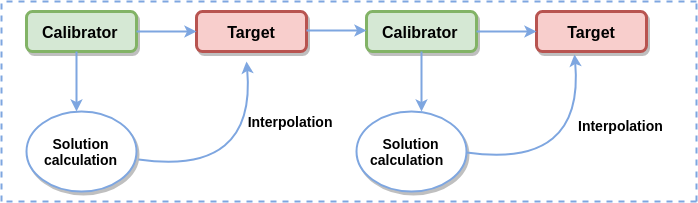
\includegraphics[width=0.7\textwidth]{images/cal4.png}
    \caption{Observation procedure and calibration using CASA}
  \label{Cal2}
\end{figure}

\begin{figure}[H]
  \centering
    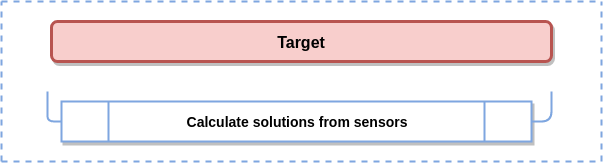
\includegraphics[width=0.7\textwidth]{images/Cal3.png}
    \caption{Observation procedure goal using machine learning}
  \label{Cal3}
\end{figure}

Figure \ref{Cal2} is shows the observation procedure of KAT-7 where the calibrator is close to the target source preferably within the range of $10^{\circ}$ to $15^{\circ}$, with the scan switching  between  the target and the calibrator \citep{kassaye2015study}. This is to minimize the phase perturbation caused by atmosphere. The calibration solutions are obtained from the phase calibrator ("green") in Figure \ref{Cal2} at different time intervals $\Delta t$ of tracking, Assuming that the calibrator PKS1613-586 has invariant characteristics (i.e known positions in the sky) during the period of observation such that the 
antenna-based  phase  gain response is zero with constant amplitude. In reality this is not always the case due to instrumental defects such as phase and amplitude drifts in the electronics of each antenna, amplitude response as a function of elevation (gain curve), and tropospheric amplitude and phase effects and other external effects. Hence, to calculate the calibration solutions, CASA consider each antenna-based gains $J_i$ and the prior information about the calibrator to perform some adjustments or estimations $G$ over time intervals $\Delta t$, such that each antenna phase gain response is zero or stable with constant amplitude. These solutions at each time interval are then temporarily interpolated using the $\textit{interp}$ parameter inside the $\textit{gaincal}$ task. 

Interpolation is a model based recovery of continuous data from discrete data with known range \citep{thevenaz2000image}. There are different methods of interpolation used, and in this Section, we only look at linear and nearest interpolation which are popular in radio calibration. Example: Assume that we have two known data points $(x_1,y_1,t_1)$ and  $(x_2,y_2,t_2)$ at time $t_1$ and $t_2$, we would like to estimate what $y$ value we would obtain at time $t$ for some point $x$ that is between $x_1$ and $x_2$. For nearest interpolation method, $y$ would be assigned to the value of the nearest point of $x$. For linear interpolation method, a line is fitted between the points $(x_1,y_1,t_1)$ and $(x_2,y_2,t_2)$  and we look to see the value of $y$ in a line for our chosen $x$ at time $t$. The points $x_1,\dots, x_n$ are called the interpolation points. The property of passing
through these points is referred to as interpolating the data and the function that interpolates the data is an interpolant \citep{levy2010introduction}. An example of interpolation is further illustrated in the following Figure \ref{int}. 

  \begin{figure}[H]
  \centering
    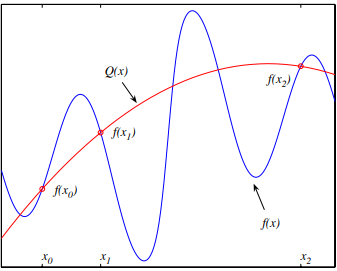
\includegraphics[width=0.5\textwidth]{images/Int.png}
    \caption{Given a function $f(x)$ with distinct points $x_0<x_1,<x_2,\dots <x_n$ at $n+1$. The interpolation problem is to construct a function $Q(x)$ that passes through these points, i.e, to find a function $Q(x)$ such that the requirements $Q(x_i)=f(x_i)$, $0\leq i\leq n$ are satisfied \citep{levy2010introduction}.}
  \label{int}
\end{figure}

 
After obtaining the solutions $G$, they are written in calibration tables and later be applied to the target source of interest $T$. The CASA task for this process is called $\textit{applycal}$ which reads the specified calibration tables, applies them to the raw/observed data column through an interpolation process at each single time unit for different time intervals $\Delta t, \Delta t_{n+1},\dots$, following the order shown in Figure \ref{Cal2}. The calibrated results are then written into the corrected column for imaging or other science processing \citep{ott2013casa}. Since CASA "calculates" the solutions using interpolation and estimation methods given some prior information about the calibrators, the goal of our experiment is to produce a model (based on the training data) that learns the behaviour and changes of the calibrator due to various external effects and be able to predict the calibration solutions of the test data with high accuracy given only the test sensors. This will help in speeding up the calibration processes and also decreasing the time duration for tracking the phase calibrator PKS1613-586 and therefore increasing time duration for tracking the target observed as shown in Figure \ref{Cal3}. 

Since the sensor data obtained from the radio telescope are of different scales, i.e, it is unstructured. a pre-processing stage before proceeding with the training of the learning algorithms is necessarily. We propose to use a scaling statistical technique called Z-score normalization or standardization. This technique gives the normalized values or range of data from the original unstructured data using the concept of mean and standard deviation \citep{patro2015normalization}. The features are rescaled such that they have properties of a standard normal distribution with mean $\mu=0$ and standard deviation $\sigma=1$. 
\begin{align}
Z=\frac{\textbf{x}- \mu}{\sigma}
\end{align}
with mean:
\begin{align*}
\mu= \frac{1}{N} \sum_{j\in N} (\textbf{x}_j),
\end{align*}

and standard deviation:
\begin{align*}
\sigma=\sqrt{ \frac{1}{N} \sum_{j\in N} (\textbf{x}_j-\mu )^2}
\end{align*}
Normalizing the features so that they are centred around 0 with a standard deviation of 1 is not only important if we are comparing measurements that have different units, but it is also a general requirement for many machine learning algorithms as this will be helpful in the prediction purpose \citep{bott2014feature}.

When training a learning algorithm  in machine learning, there are two main things that might happen as described in Section \ref{comp}, namely overfitting and underfitting. To avoid these, we split our data into two subsets, i.e, training and testing data sets using the $\textit{scikit-learn}$ train-test split strategy \citep{buitinck2013api}. 

  \begin{figure}[H]
  \centering
    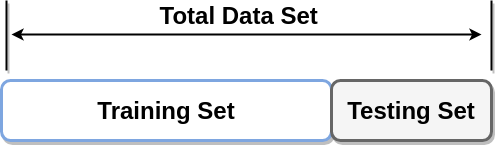
\includegraphics[width=0.7\textwidth]{images/t_s.png}
    \caption{This is a train-test split strategy where a data matrix is randomly splitted into training and testing  subsets.}
  \label{ts}
\end{figure}

From the Figure \ref{ts}, now that our data is normalized, we perform a 80 $\%$ training and 20$\%$ testing split. The training set contains a known output and the model will learn on this data in order to be generalized to other data later on. We have the test dataset in order to test our model's prediction on this subset.
 
Model training in machine learning requires tuning of the  hyper-parameters which determines the behaviour of the learning algorithm and hence the performance
of the resulting model on unseen data. This involves finding the best combination of hyper-parameters with respect to the user specified criterion \citep{buitinck2013api}. For this task, we make use of a randomized search cross validation (RandomizedSearchCV) function by $\textit{scikit-learn}$ library. This library provide efficient and well-established machine learning tools within
a programming environment that is accessible to non-machine learning experts and reusable in various scientific areas \citep{buitinck2013api}. In randomized search cross validation algorithm, not all hyper parameters are tried out, instead it samples a fixed number of hyper-parameters from a specified probability distribution. i.e, Given a set of parameters $p_i$ each with $N_i$ different values, search all combinations $\prod_i N_i$ with random sampling.


   \begin{figure}[H]
  \centering
    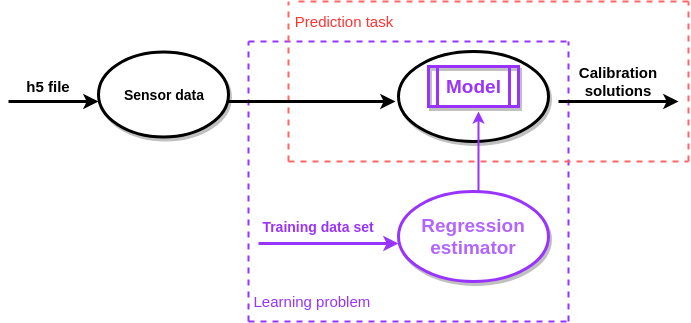
\includegraphics[width=0.7\textwidth]{images/RegressionEST.png}
    \caption{Regression learning diagram showing how we build a regression model estimator by taking in an observation file as input and extract the sensor data per calibrator scan to obtain an accurate model which predicts calibration solutions.}
  \label{DD}
  \end{figure} 


  \begin{table}[H]
\begin{center}
\begin{tabular}{| c | c | c | c | c | c |  }
\hline
 \multicolumn{6}{ |c|}{\textbf{Decision tree estimator $p_i$}} \\ \hline
splitter & max features & min sample split & min sample leaf & max depth & cv\\ \hline
[best,random]&[log2& $\{p_i: 30 \leq p_i \leq 60 \}$& $\{p_i: 7 \leq p_i \leq 14 \}$  & $\{p_i: 700 \leq p_i \leq 1389 \}$ & 10\\ 
&sqrt& & &  &\\
&auto]& & &  &\\ \hline

\end{tabular}
\end{center}
\caption{Decision-hyper-parameters} \label{DC_table}
\end{table}


  \begin{table}[H]
\begin{center}
\begin{tabular}{| c | c | c | c | c |  }
\hline
 \multicolumn{5}{ |c|}{\textbf{Random forest estimator $p_i$}} \\ \hline
 n-estimators &max features & max depth & min sample leaf& cv\\ \hline
$\{p_i: 100 \leq p_i \leq 1200 \}$&[log2& $\{p_i: 20 \leq p_i \leq 200 \}$  & $\{p_i: 3 \leq p_i \leq 50 \}$ & 10\\ 
&sqrt& & &  \\
&auto]& & &\\ \hline

\end{tabular}
\end{center}
\caption{Random forest hyper-parameters} \label{RF_table}
\end{table}


 \begin{table}[H]
\begin{center}
\begin{tabular}{| c | c | c | c | c |  }
\hline
 \multicolumn{5}{ |c|}{\textbf{Extremely randomized estimator $p_i$}} \\ \hline
 n-estimators &max features & max depth & min sample leaf& cv\\ \hline
$\{p_i: 100 \leq p_i \leq 1200 \}$&[log2 & $\{p_i: 20 \leq p_i \leq 200 \}$  & $\{p_i: 3 \leq p_i \leq 50 \}$ & 10\\ 
&sqrt& & &  \\
&auto]& & &  \\ \hline

\end{tabular}
\end{center}
\caption{Extremely randomized tree hyper-paramaters}\label{EX_table}
\end{table}

Note that since the random forest estimator \ref{RF_table} and extremely randomized estimator 
\ref{EX_table} are tree based algorithms, they share the same hyper-parameters as the decision tree estimator \ref{DC_table}. Where 
\begin{enumerate}
\item \textit{splitter}: is the strategy used to choose the split at decision node, with $p_i$ best representing the best split and random representing the random split.

\item \textit{max features}: defines the maximum number of features to be considered in the tree when making the best split. The best parameter $p_i$ to choose from are : 
\begin{itemize}
\item if $p_i$ is $\log_2$ then the maximum features is  $\log_2\left(\textit{max features} \right)$

\item if $p_i$ is sqrt then the maximum features is $\sqrt{\textit{max features}}$ 
\item if $p_i$ is auto, then this will simply take all the features which make sense in every tree. Here we simply do not put any restrictions on the individual tree. 
\end{itemize}
\item \textit{min sample split}: denotes the minimum number of samples required for for a split in each decision node.
\item \textit{max depth}: denotes the maximum depth of the tree, i.e determine how deep the tree should expand. If None parameter is given, then nodes are expanded until all leaves are pure or until all leaves contain less than min samples split samples.

\item \textit{min sample leaf}: denotes the number of samples required for a node to be a terminal node(leaf node).
\item \textit{n-estimator}: denotes  the number of trees  to be built before taking the maximum voting or averages of predictions. Higher number of trees gives better performance but makes decrease the speed of processing power.
\item \textit{cv}: denotes the cross validation generator inside RandomizedSearch which determines the cross validation strategy, if $p_i$ is an integer, then the number of folds in a KFold are specified \citep{pedregosa2011scikit}. 
\end{enumerate}


\begin{table}[H]
\begin{center}
\begin{tabular}{| c | c | c | c | c | c |  }
\hline
 \multicolumn{6}{ |c|}{\textbf{K-nearest neighbor estimator $p_i$}} \\ \hline
n-neighbors & weights & algorithm & leaf size & p & cv\\ \hline
$\{p_i: 20 \leq p_i \leq 200 \}$&[uniform,distance]&  [auto&$\{p_i: 30 \leq p_i \leq 150 \}$  & [2,3] & 10\\
&&  ball-tree&  &  &\\
&&  kd-tree&  &  &\\ 
&&  brute]&  &  &\\ \hline
\end{tabular}
\end{center}
\caption{K-nearest neigbor hyper-parameters} \label{KNN_table}
\end{table}

One of the most attractive features of the K-nearest neighbor algorithm is that is simple to understand and easy to implement. As shown in Table \ref{KNN_table}, few hyper- parameters $p_i$ are tried out, hence it is called a lazy learning algorithm. 

\begin{enumerate}

\item \textit{n-neighbors}: denotes the number of the  K nearest neighbors of the unknown observation. When K is small, we are restraining the region of a given prediction and forcing our predictor be limited in seeing the overall distribution, and a higher K averages more voters in each prediction and hence is more resilient to outliers.  
\item \textit{weights}: denotes the weight contribution of each point to the prediction of a query point in the local neighborhood.  
\begin{itemize}

\item if weight is uniform, then all points are weighted  equally.
\item if weight is distance, then the weights proportional to the inverse of the distance from the query point is assigned.  
\end{itemize}
\item \textit{algorithm}: specifies which algorithm  should be used to compute the nearest neighbors and takes in values like:
\begin{itemize}

\item if algorithm is auto, then the algorithm attempts to determine the best approach from the training data.

\item ball-tree, kd-tree algorithm are used to implement ball tree algorithm. These data structures are used for fast high-dimensional nearest-neighbor searches.  
\item brute algorithm is used to implement brute-force search algorithm. 
\end{itemize}
\item \textit{leaf size} leaf size passed to ball-tree or kd-tree approach for finding k-nearest neighbors in.

\item \textit{p} denotes the power parameter for the Minkowski metric \citep{pedregosa2011scikit}.
\end{enumerate}

With the number of iterations $\text{n-iter}=50$ RandomizedSearchCV algorithm used to search through, the best estimator obtained, which is the instantiation
mechanisms of objects and exposes a fit method for learning a model from
training data for each learning algorithm is:   
\begin{tcolorbox}
\begin{verbatim}

DecisionTreeRegressor(criterion='mse', 
                      max_depth=890,       
                      max_features='log2',
                      max_leaf_nodes=None,
                      min_impurity_split=1e-07,
                      min_samples_leaf=13, 
                      min_samples_split=30,
                      min_weight_fraction_leaf=0.0, 
                      presort=False, 
                      random_state=0,
                      splitter='best')
\end{verbatim}
\end{tcolorbox}
\begin{figure}[H]
\centering 
\begin{tabular}{l*{8}{c}r}
\hline
            & max-depth &max features&min samples leaf & min samples split  &splitter& score \\
\hline
optimized $p_i$  & 890 & $\log_2$ & 13 & 30 & best&0.686  \\
\end{tabular}
\caption{Decision tree optimized hyper-parameters }
\end{figure}
\begin{tcolorbox}
\begin{verbatim}
RandomForestRegressor(bootstrap=True,
                      criterion='mse',
                      max_depth=90,
                      max_features='auto',
                      max_leaf_nodes=None,
                      min_impurity_split=1e-07,
                      min_samples_leaf=3,
                      min_samples_split=2,
                      min_weight_fraction_leaf=0.0,
                      n_estimators=700,
                      n_jobs=1, 
                      oob_score=0,
                      random_state=0,
                      verbose=0,
                      warm_start=False)
\end{verbatim}
\end{tcolorbox}
\begin{figure}[H]
\centering 
\begin{tabular}{l*{8}{c}r}
\hline
            & max-depth &max features&min samples leaf &n-estimators & score \\
\hline
optimized $p_i$  & 90 & auto & 3 & 700 & 0.902 \\
\end{tabular}
\caption{Random forest optimized hyper-parameters }
\end{figure}
\begin{tcolorbox}
\begin{verbatim}
KNeighborsRegressor(algorithm='brute',
                    leaf_size=30, 
                    metric='minkowski',
                    metric_params=None,
                    n_jobs=1,
                    n_neighbors=20,
                    p=3,
                    weights='distance')
\end{verbatim}
\end{tcolorbox}
\begin{figure}[H]
\centering 
\begin{tabular}{l*{8}{c}r}
\hline
            & algorithm &n-neighbors&p &weights \\
\hline
optimized $p_i$ &brute&20& 3 & distance \\
\end{tabular}
\caption{KNN optimized hyper-parameters }
\end{figure}
\begin{tcolorbox}
\begin{verbatim}
ExtraTreesRegressor(bootstrap=False, 
                    criterion='mse',
                    max_depth=90,
                    max_features='auto',
                    max_leaf_nodes=None,
                    min_impurity_split=1e-07,
                    min_samples_leaf=3,
                    min_samples_split=2, 
                    min_weight_fraction_leaf=0.0,
                    n_estimators=700,
                    n_jobs=1, 
                    oob_score=0,
                    random_state=0,
                    verbose=0, warm_start=False)
\end{verbatim}
\end{tcolorbox}

\begin{figure}[H]
\centering 
\begin{tabular}{l*{8}{c}r}
\hline
            & max-depth &max features&min samples leaf &n-estimators& score \\
\hline
optimized $p_i$  & 90 & auto & 3 & 700 &0.905 \\
\end{tabular}
\caption{Extremely randomized tree optimized hyper-parameters }
\end{figure}

\subsection{Feature importance}
Random forests and extremely randomised are well established ensemble of trees models that not only produce good predictive performance, but also provide rich feature importance information \citep{kazemitabar2017variable}. Generally, importance provides a score that indicates how  valuable each feature was in the construction of the decision trees within the model. These scores are used for model selection: predictors with high-ranking scores, the more a feature  is used to make key decisions with decision trees and other further investigation \citep{pedregosa2011scikit}. Importance is calculated for a single decision tree by the amount that each split point improves the performance measure, weighted by the number of observations the node is responsible for. The performance measure can be the average of the impurity reductions over all nodes in the tree where a split was made on that variable, with impurity reductions weighted to account for the size of the node \citep{kazemitabar2017variable}.

\begin{figure}[H]
  \centering
    \includegraphics[width=0.8\textwidth]{images/FeatureSpace.eps}
    \caption{Feature importance}
    \label{FI}
\end{figure}
Figure \ref{FI} is showing the importance of each feature in each learning algorithm. i.e the values with hight contribution in building an accurate model. We observe that the environmental features air temperature, relative humidity, wind speed, wind direction and air pressure are highly ranked in than the pointing sensors. The pointing features are ranked second best with the telescope elevation sensors being higher than the telescope azimuth sensors. 

\section{Results}
\label{sec3}
This section shows the plots of the predictions for the decision tree, random forest, extremely randomised trees and the K-nearest neighbor. The algorithms are run couple of times on the learning sample and tested on the test samples to estimate the errors. In the following, we report the accuracy measure obtained for each method when evaluating on testing dataset. In every model there are four plots each for amplitude and phase h $\&$ v polarization. The $y-axis$ in each subplot is the predicted gain amplitude  and phase solutions, the $x-axis$ is the ground truth gain amplitude and phase solution corresponding to the testing sensor data. Note that the two cluster grouping of points in the predicted vs ground truth amplitude Figures : \ref{B1}, \ref{B2}, \ref{B3}, \ref{B4}, \ref{B5}, \ref{B6}, \ref{B7} is due to the sinusoidal variation of the amplitude solutions as shown in Figure \ref{amp}. In the testing of gain and phase solutions, we used the appropriate regression evaluation methods : rmse, rmae, r2score and the explained variance. The evaluation results obtained from the extremely randomized trees, random forest, and K-nearest neighbor are accurate with h polarization rmse $\approx 0.3$  and v polarization $\approx 0.2$ for gain phase prediction as shown in Figures Figures \ref{A2}, \ref{A3}, \ref{A4}, \ref{A5}, \ref{A6}, \ref{A7}, \ref{A7}. The gain amplitude prediction is more accurate for random forest and extremely randomized tree on h $\&$ v polarization with rmse error  $\approx 0.02$ much less than gain phase prediction as shown in Figures \ref{B2}, \ref{B3}, \ref{B6}, \ref{B7}. We further observe that majority of the predictions stay near the ground truth values with coefficient of determination $R^2$ score converging to 1.
\begin{figure}[H]
   \centering
    \begin{subfigure}[t]{0.52\textheight}
        
        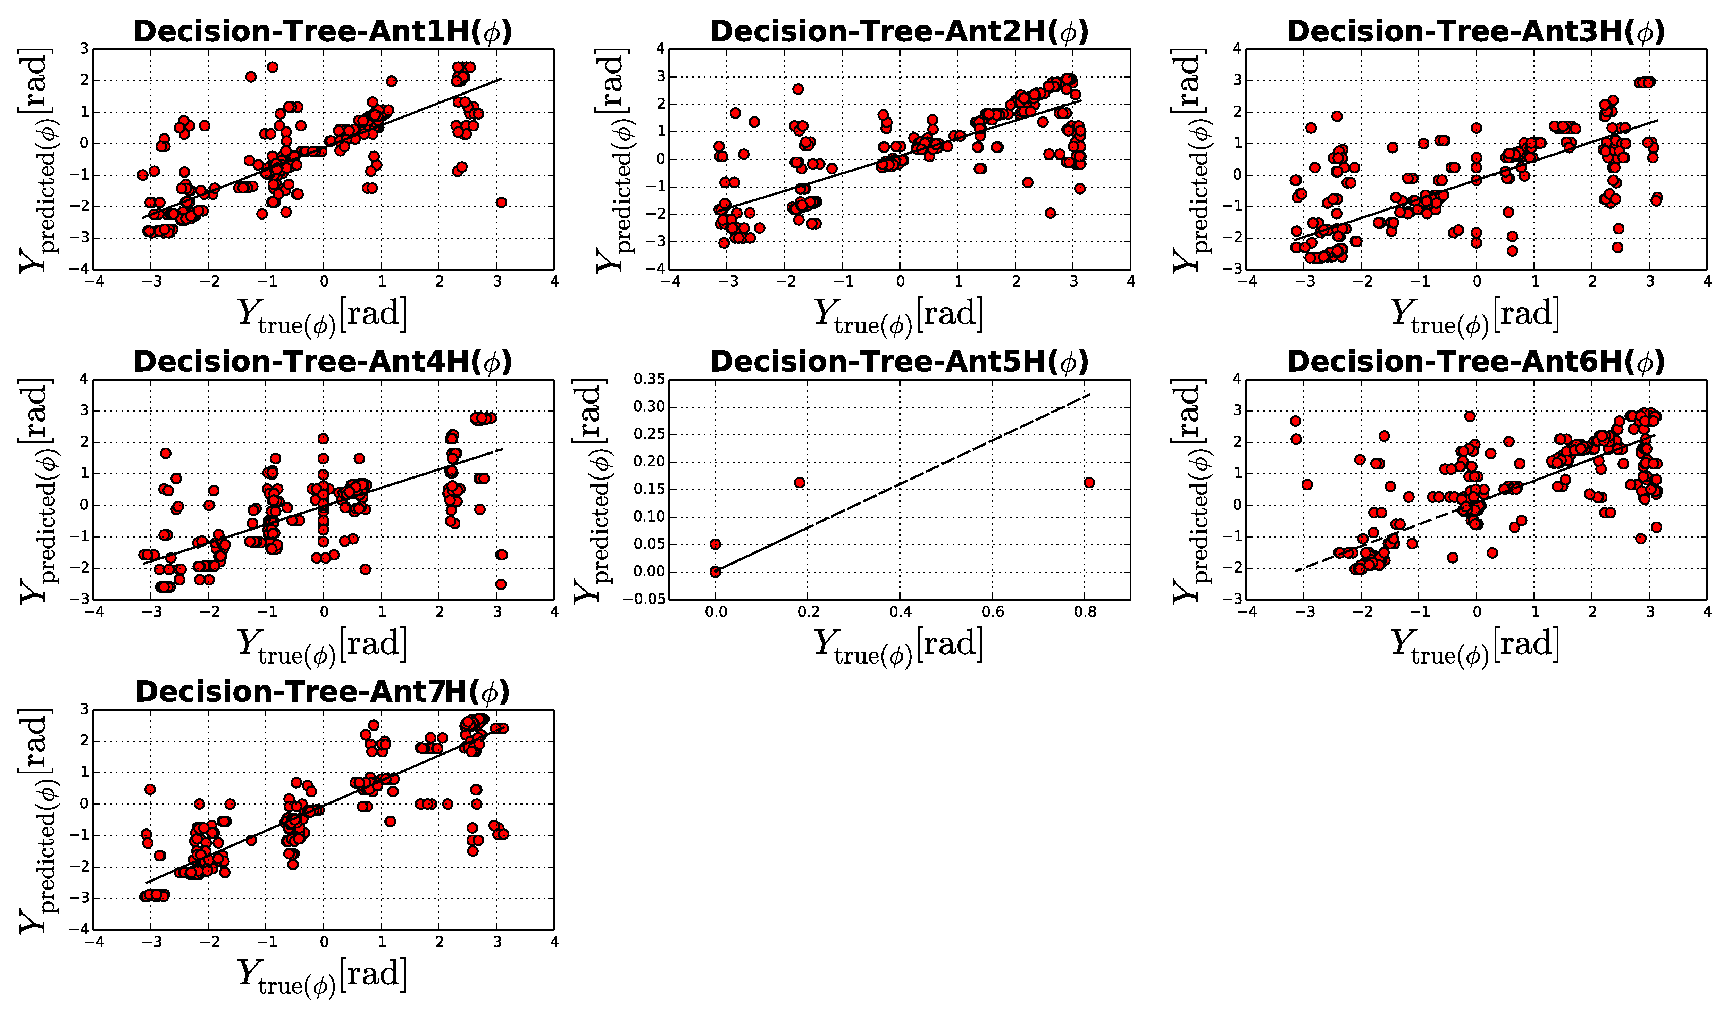
\includegraphics[width=\textwidth]{images/Decision-TreeHphase.eps} 
        \caption{Phase gain solutions for h polarization}
         \label{A}
    \end{subfigure}
    
      \begin{subfigure}[t]{0.52\textheight}
       
        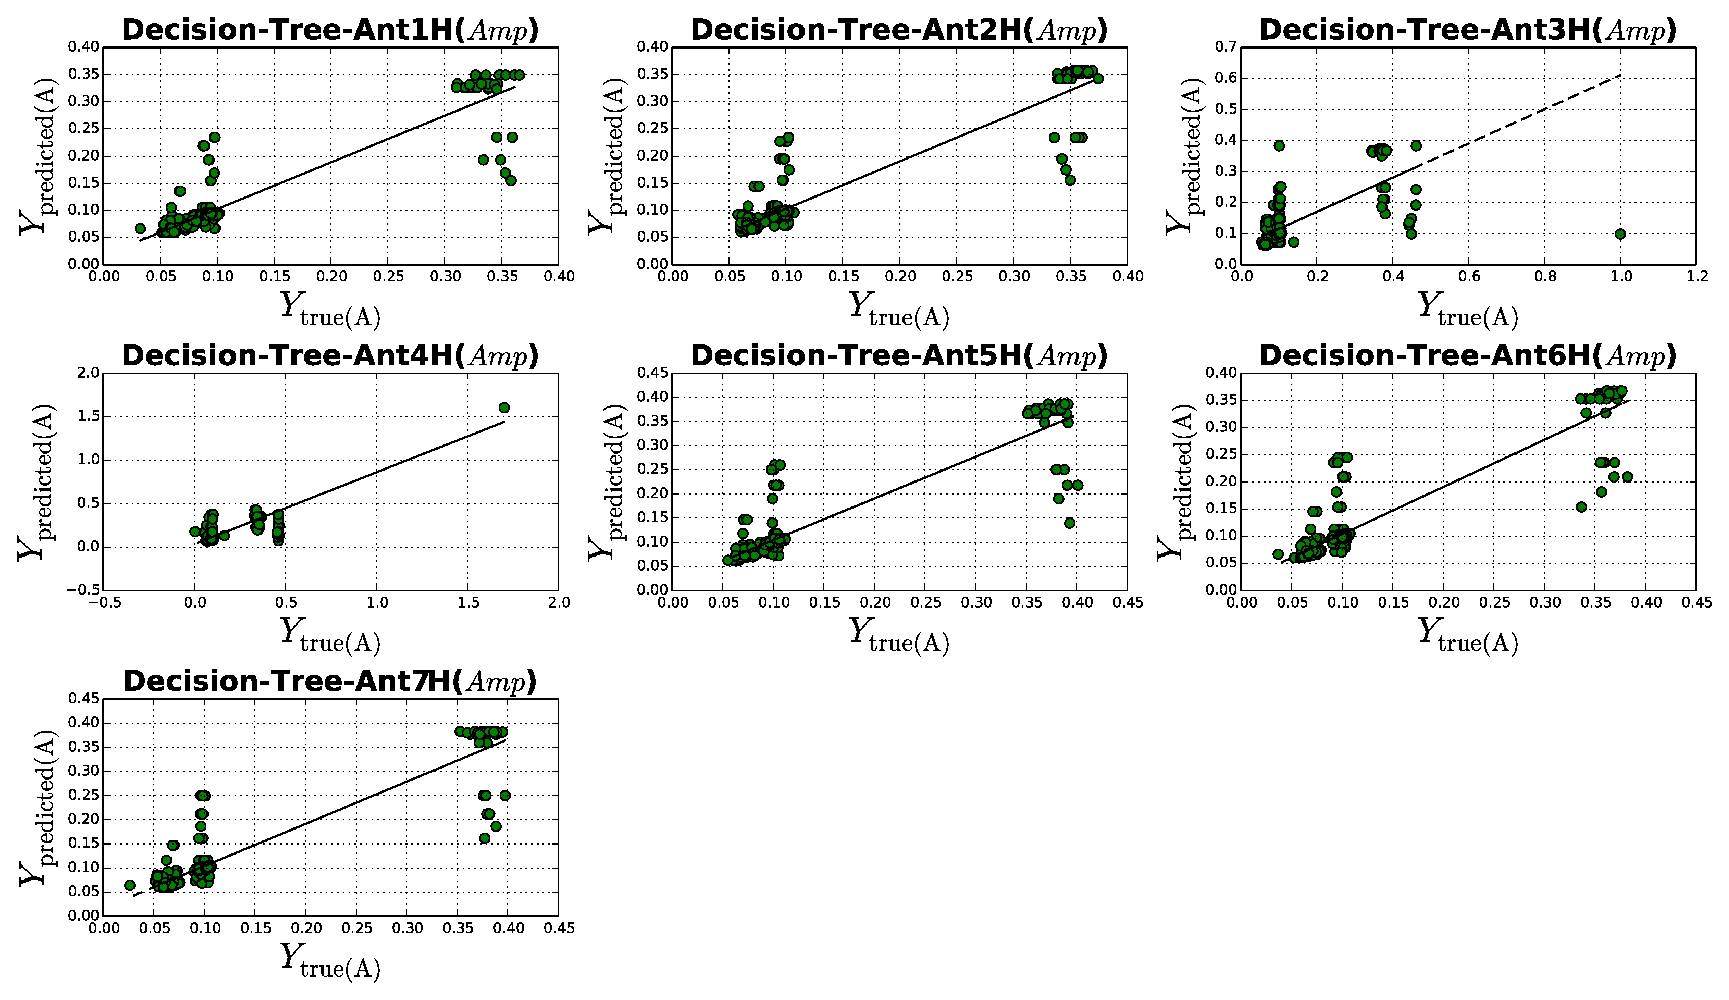
\includegraphics[width=\textwidth]{images/Decision-TreeHamp.eps} 
        \caption{Amplitude gain solutions for h polarization.}
         \label{B}
    \end{subfigure}
    \caption{Demonstrates the results obtained from the decision tree learning algorithm with randomized search optimization algorithm. (\subref{A}) and (\subref{B}) is the predicted phase gain solutions $\textbf{Y}_{predicted}$ by the learning algorithm vs the true phase gain solutions $\textbf{Y}_{true}$ (CASA) for h polarization in radians. }
    \end{figure}
  
\begin{figure}[H]
   \centering
    \begin{subfigure}[t]{0.52\textheight}
        
        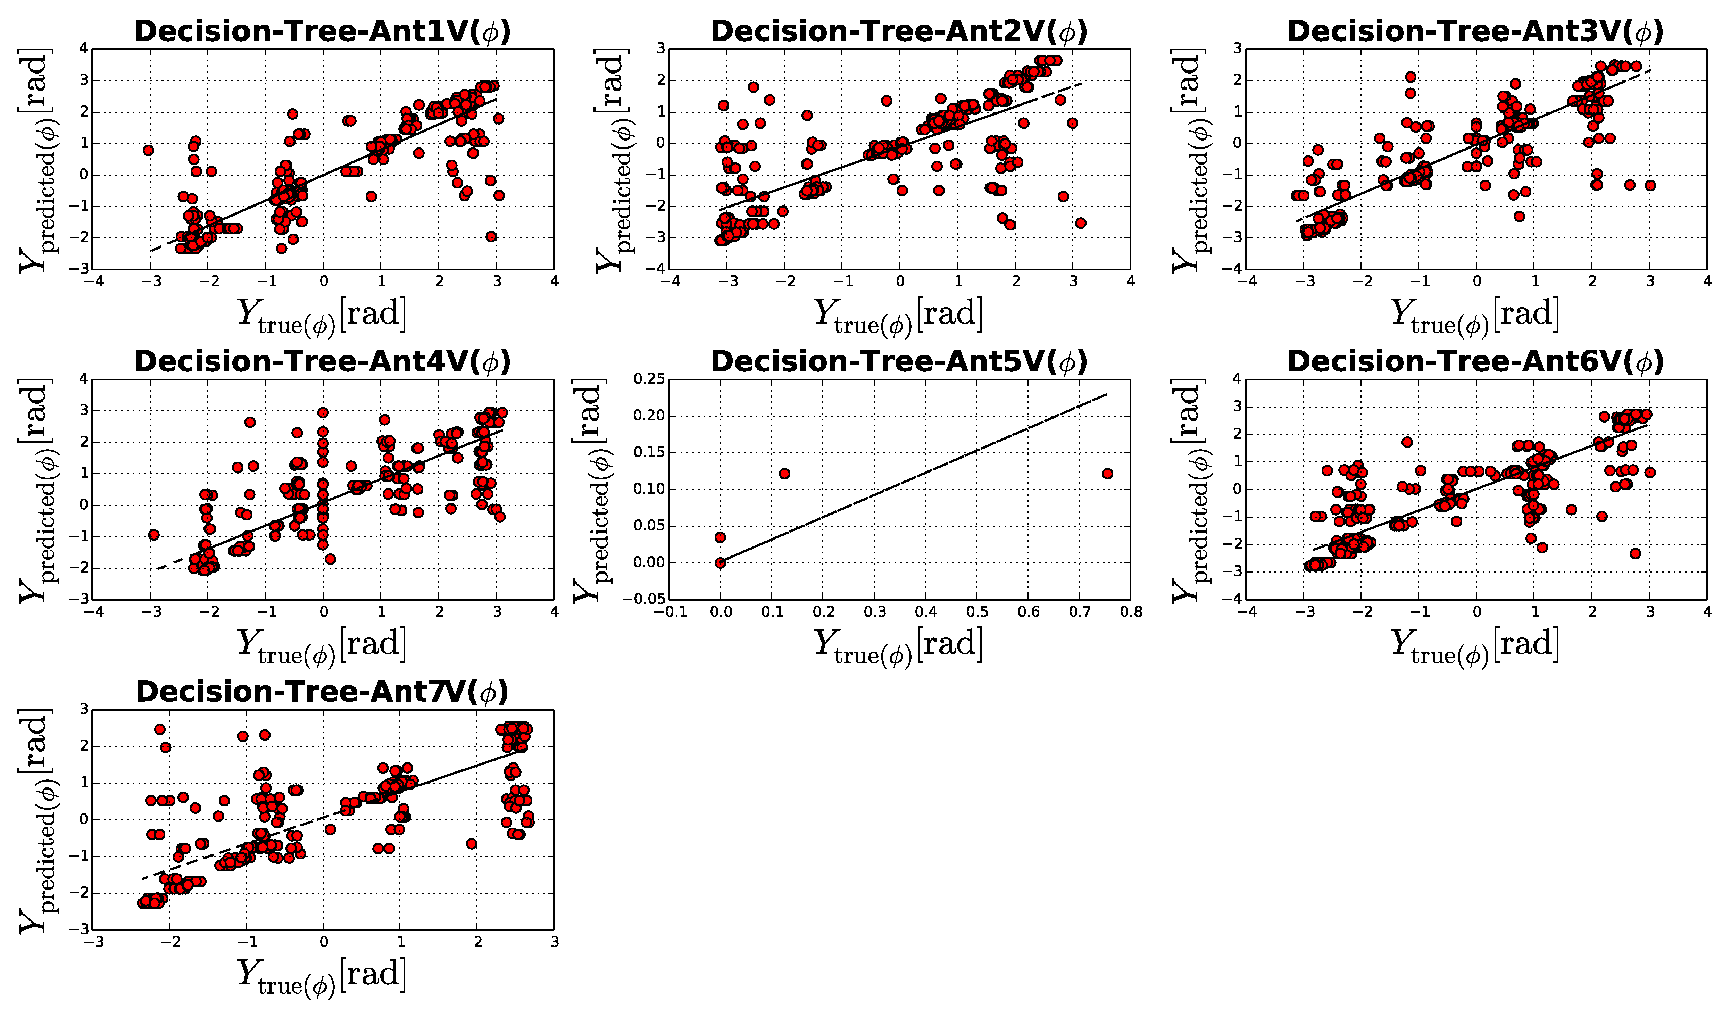
\includegraphics[width=\textwidth]{images/Decision-TreeVphase.eps} 
        \caption{Phase gain solutions for v polarization}
         \label{A1}
    \end{subfigure}
    
      \begin{subfigure}[t]{0.52\textheight}
       
        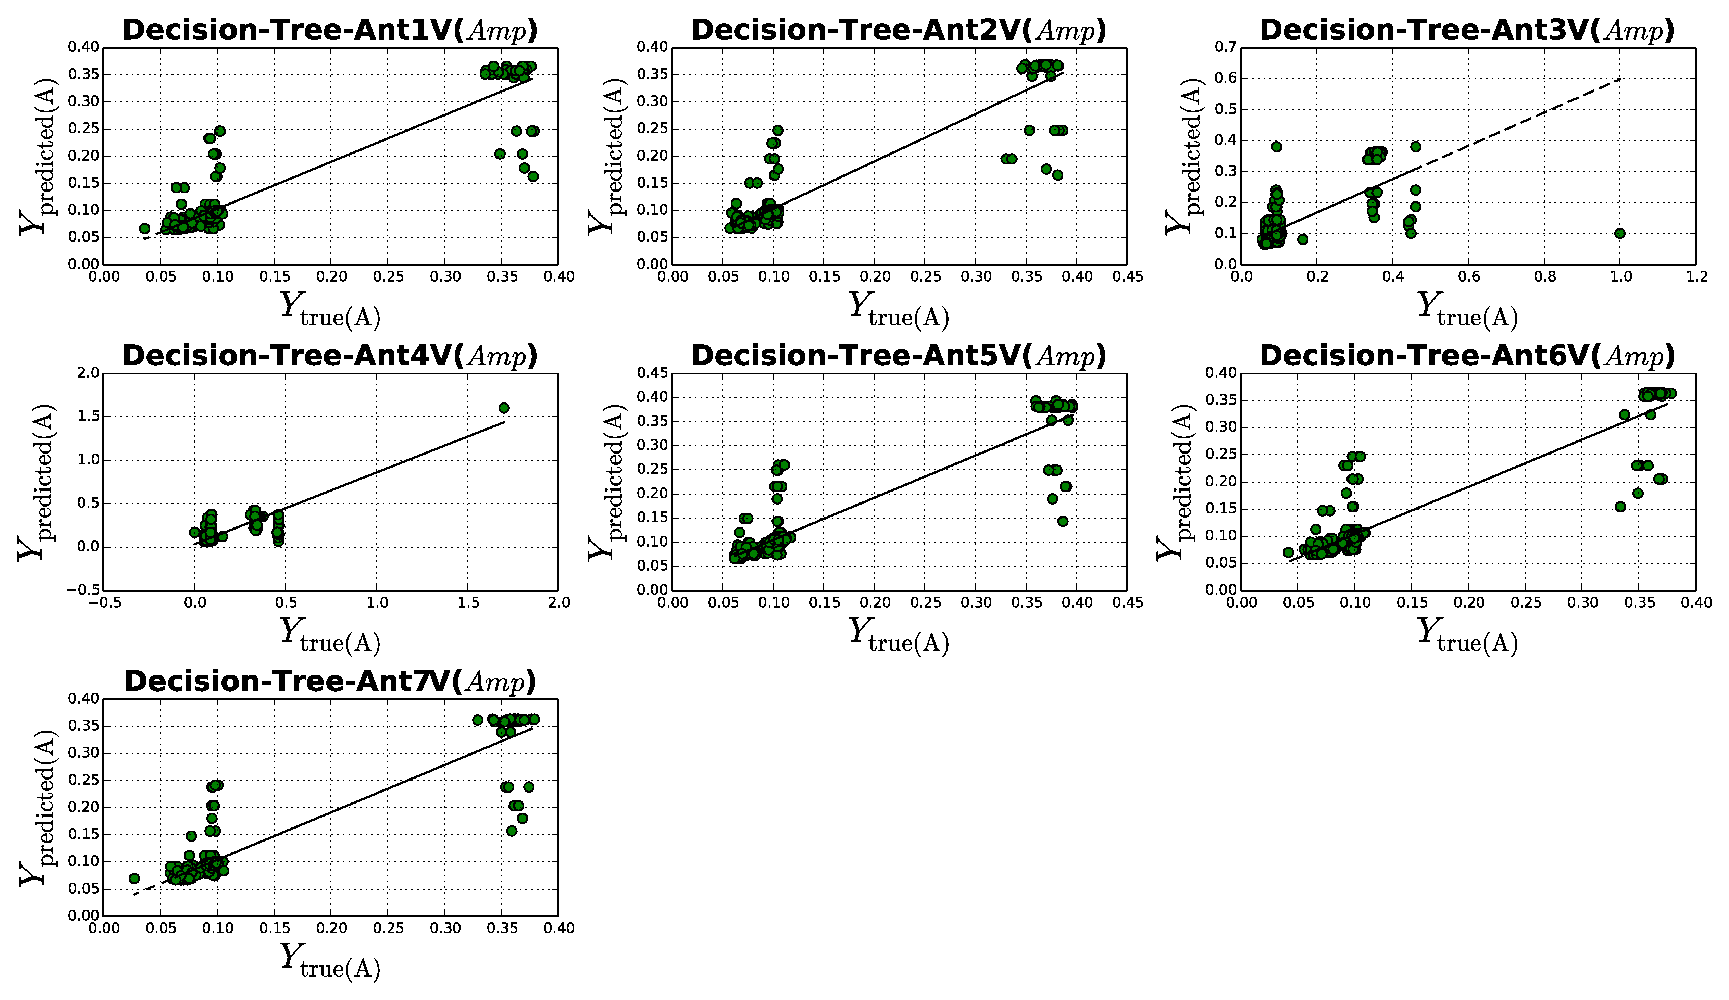
\includegraphics[width=\textwidth]{images/Decision-TreeVamp.eps} 
        \caption{Amplitude gain solutions for v polarization} 
        \label{B1}
    \end{subfigure}
    \caption{Demonstrates the results obtained from the decision tree learning algorithm with randomized search optimization algorithm. (\subref{A1}) and (\subref{B1}) is the predicted phase gain solutions $\textbf{Y}_{predicted}$ by the learning algorithm vs the true phase gain solutions $\textbf{Y}_{true}$ (CASA) for v polarization.}
    \end{figure}
    
\begin{table}[H]
\label{T:equipos}
\begin{center}
\scalebox{0.7}{
\begin{tabular}{| c | c | c | c | c |}
\hline
Antenna & \multicolumn{4}{ c |}{\textbf{Decision tree Phase}}  \\ 
\cline{2-5}
&Rmse & Rmae & R2score &Explained $\sigma^2$\\
\hline
Uniform average-H &0.573 & 0.417 & 0.820   & 0.821 \\ 
Uniform average-V &0.435 & 0.367 & 0.879    & 0. 879\\ \hline
 & \multicolumn{4}{ c |}{\textbf{Decision tree Amplitude}}  \\ 
\cline{1-5}
\hline
Uniform average-H &0.043 & 0.109 & 0.835   & 0.835 \\ 
Uniform average-V &0.043 & 0.109 & 0.831    & 0.831\\\hline
\end{tabular}}
\end{center}
\caption{The table shows the performance of the decision tree algorithm in predicting the amplitude and phase gain solutions for both h and v polarizations. The values shown represents uniform average of all KAT-7 antennas, i.e, all outputs measures are averaged with uniform weight. Majority of the predictions stay near the ideal truth values with rmse \ref{MSE} and rmae \ref{MAE}  $\approx <$ 0.5, $R^2$ \ref{R2score} and explained variance $V$ \ref{ExV} are converging to 1.}
\end{table}

\subsection{Random forest-RUN}
\begin{figure}[H]
   \centering
    \begin{subfigure}[t]{0.52\textheight}
        
        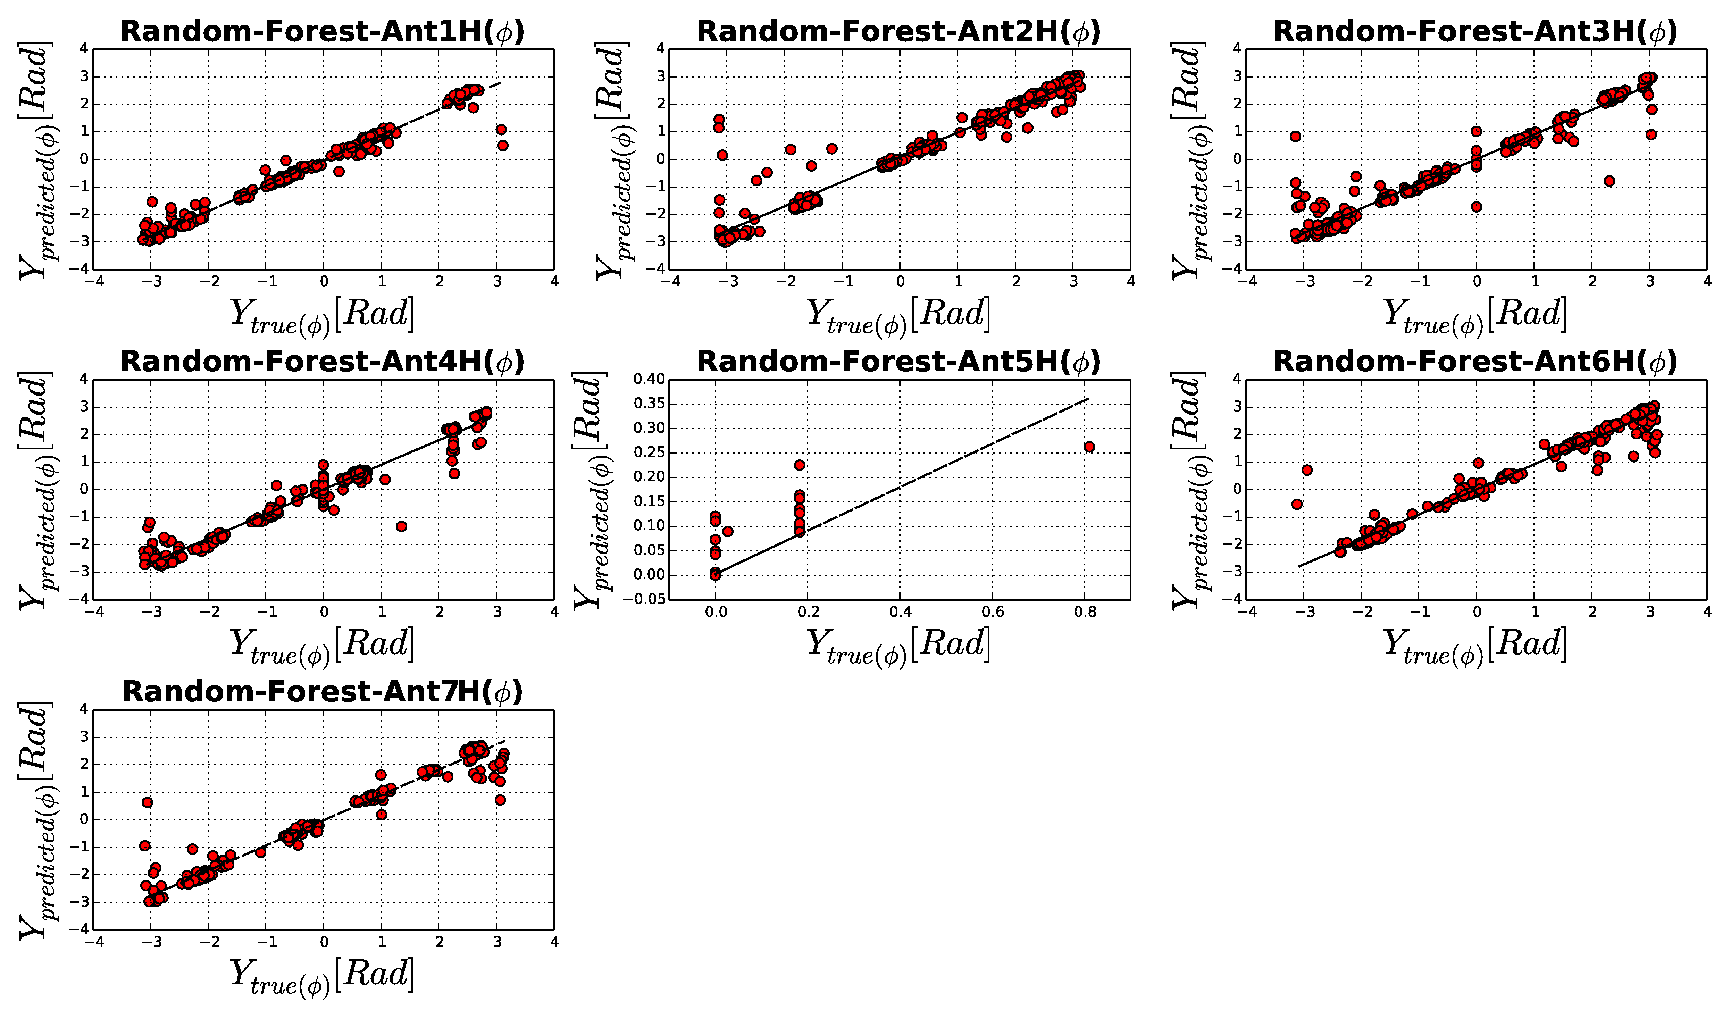
\includegraphics[width=\textwidth]{images/Random-ForestHphase.eps} 
        \caption{Phase gain solutions for h polarization} \label{A2}
    \end{subfigure}
    
      \begin{subfigure}[t]{0.52\textheight}
       
        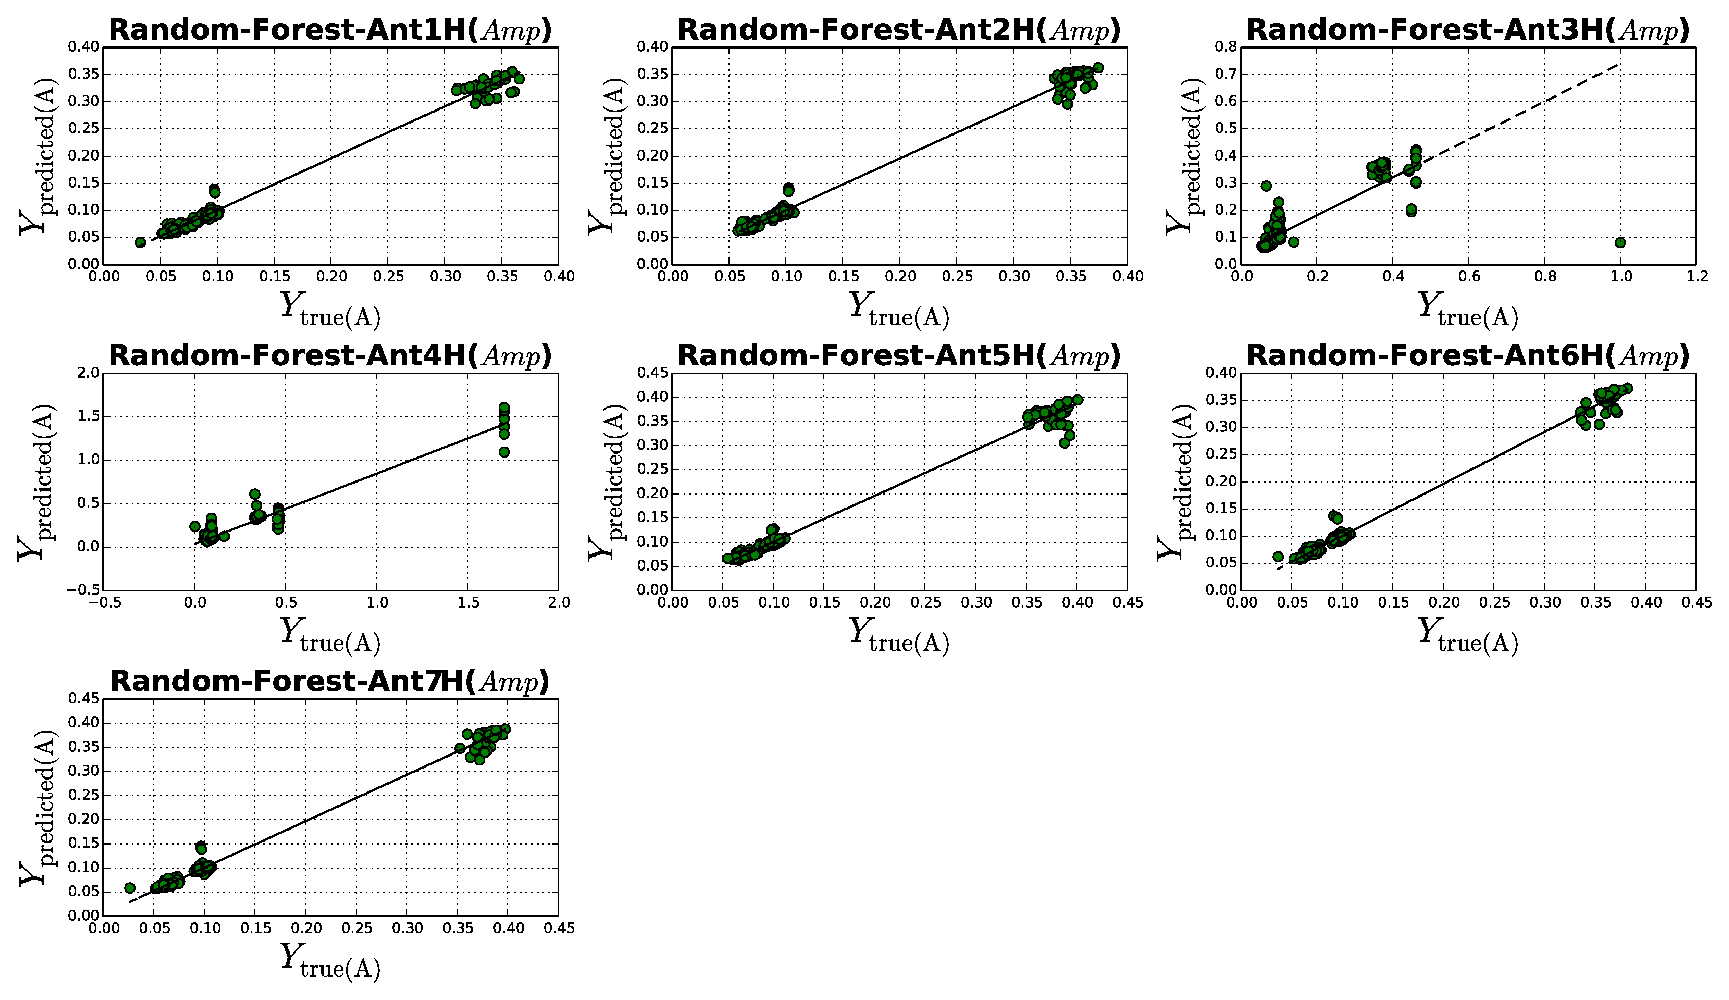
\includegraphics[width=\textwidth]{images/Random-ForestHamp.eps} 
        \caption{Amplitude gain solutions for h polarization} \label{B2}
    \end{subfigure}
    \caption{Demonstrates the results obtained from the random forest learning algorithm with randomized search optimization algorithm. (\subref{A2}) and (\subref{B2}) is the predicted phase gain solutions $\textbf{Y}_{predicted}$ by the learning algorithm vs the true phase gain solutions $\textbf{Y}_{true}$ (CASA) for h polarization in radians.}
    \end{figure}
    
\begin{figure}[H]
   \centering
    \begin{subfigure}[t]{0.52\textheight}
        
        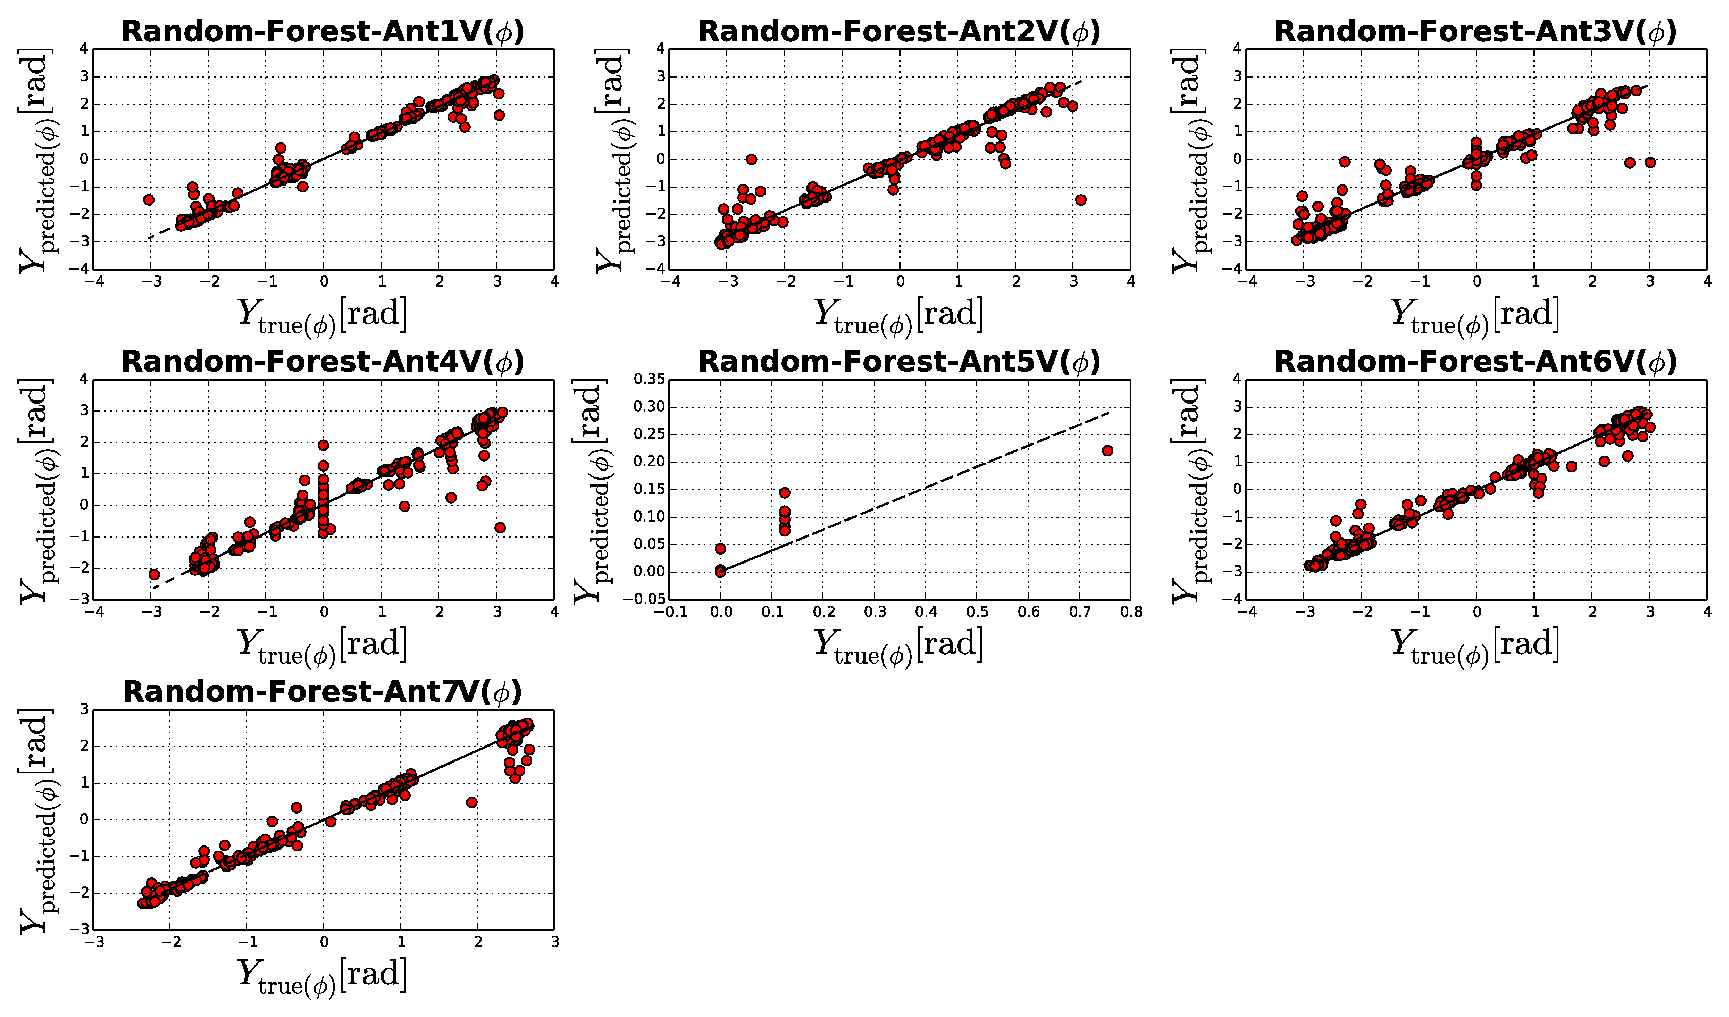
\includegraphics[width=\textwidth]{images/Random-ForestVphase.eps} 
        \caption{Phase gain solutions for v polarization} \label{A3}
    \end{subfigure}
    
      \begin{subfigure}[t]{0.52\textheight}
       
        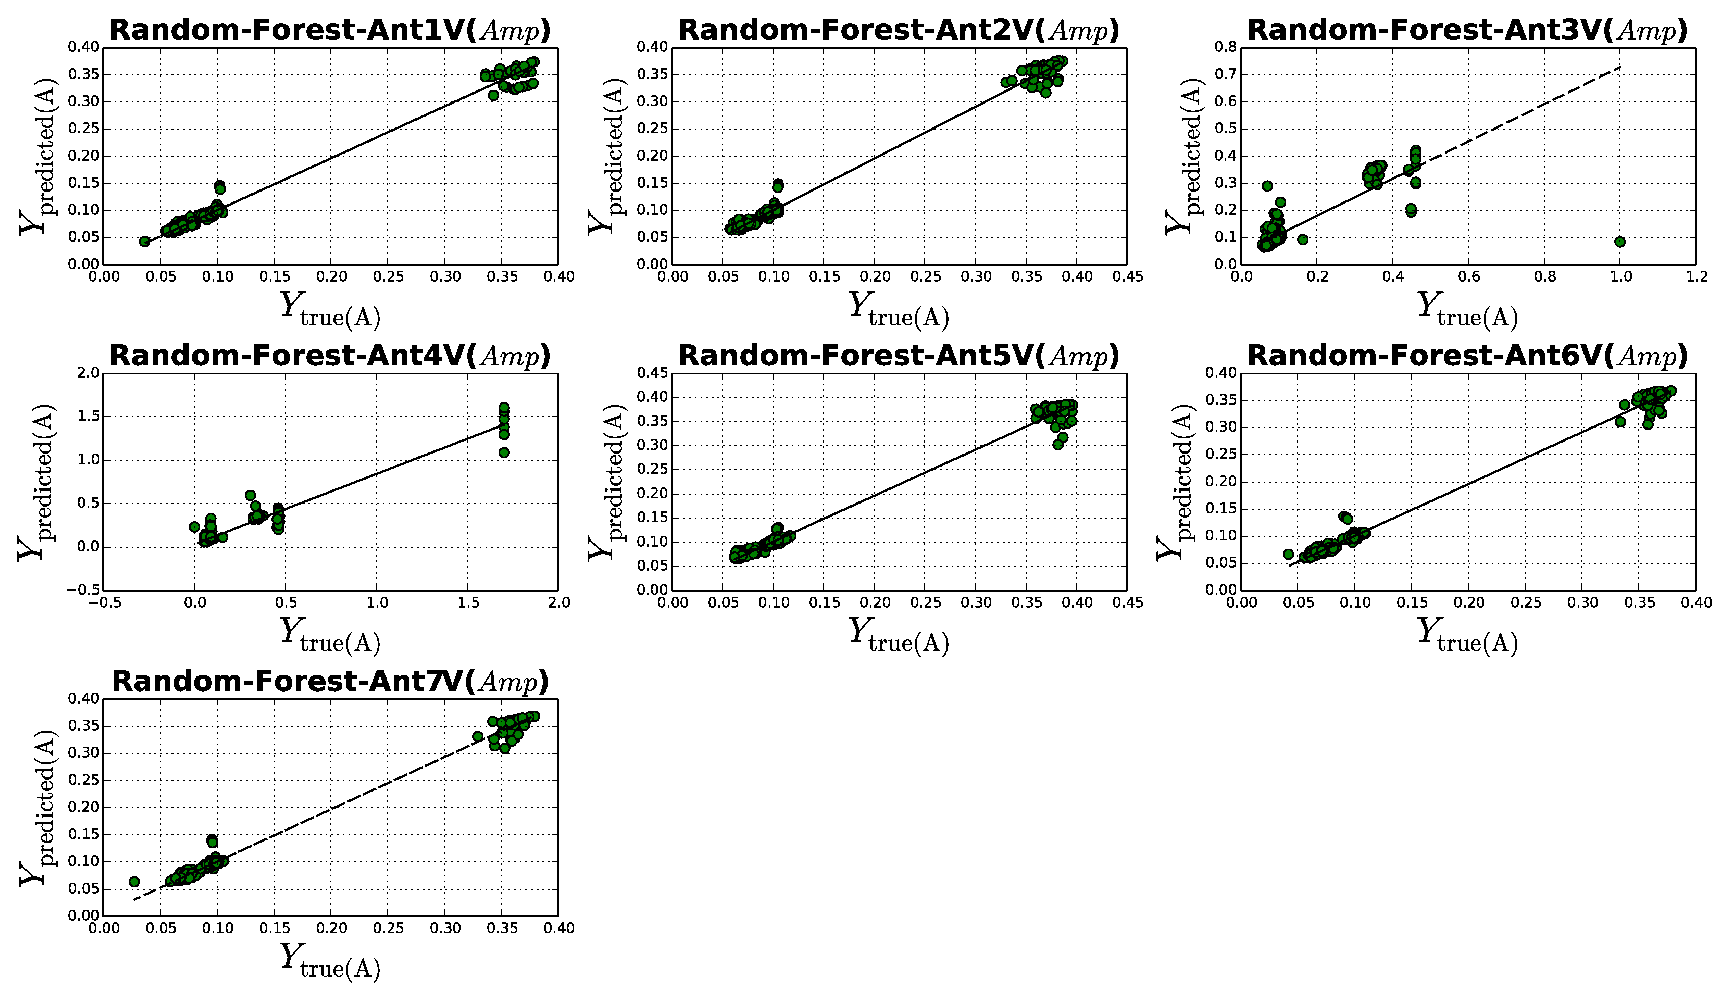
\includegraphics[width=\textwidth]{images/Random-ForestVamp.eps} 
        \caption{Amplitude gain solutions for v polarization} \label{B3}
    \end{subfigure}
    \caption{Demonstrates the results obtained from the random forest learning algorithm with randomized search optimization algorithm. (\subref{A3}) and (\subref{B3}) is the predicted phase gain solutions $\textbf{Y}_{predicted}$ by the learning algorithm vs the true phase gain solutions $\textbf{Y}_{true}$ (CASA) for v polarization in radians. }
    \end{figure} 
   
\begin{table}[H]
\begin{center}
\scalebox{0.7}{
\begin{tabular}{| c | c | c | c | c |}
\hline
Antenna & \multicolumn{4}{ c |}{\textbf{Random forest Phase}}  \\ 
\cline{2-5}
& Rmse & Rmae & R2score & Explained $\sigma^2$\\
\hline
 Uniform average-H &0.368 & 0.352 & 0.912   & 0.912 \\ 
Uniform average-V &0.256 & 0.311 & 0.939   & 0. 939\\ \hline
 & \multicolumn{4}{ c |}{\textbf{Random forest Amplitude}}  \\ 
\cline{1-5}
\hline
Uniform average-H &0.028 & 0.087 & 0.918   & 0.919 \\ 
Uniform average-V &0.028 & 0.088 & 0.916    & 0. 917\\ \hline

\end{tabular}}
\end{center}
\caption{The table shows the performance of the random forest algorithm in predicting the amplitude and phase  gain solutions for both h and v polarizations. The values shown represents the uniform average of all KAT-7 antennas, i.e, all outputs measures are averaged with uniform weight. Majority of the predictions stay near the ideal truth values with rmse \ref{MSE} and rmae \ref{MAE}  $\approx <$ 0.5, $R^2$ \ref{R2score} and explained variance V \ref{ExV} are converging to 1.}
\end{table}

\subsection{K-nearest neighbor-RUN}
\begin{figure}[H]
   \centering
    \begin{subfigure}[t]{0.52\textheight}
        
        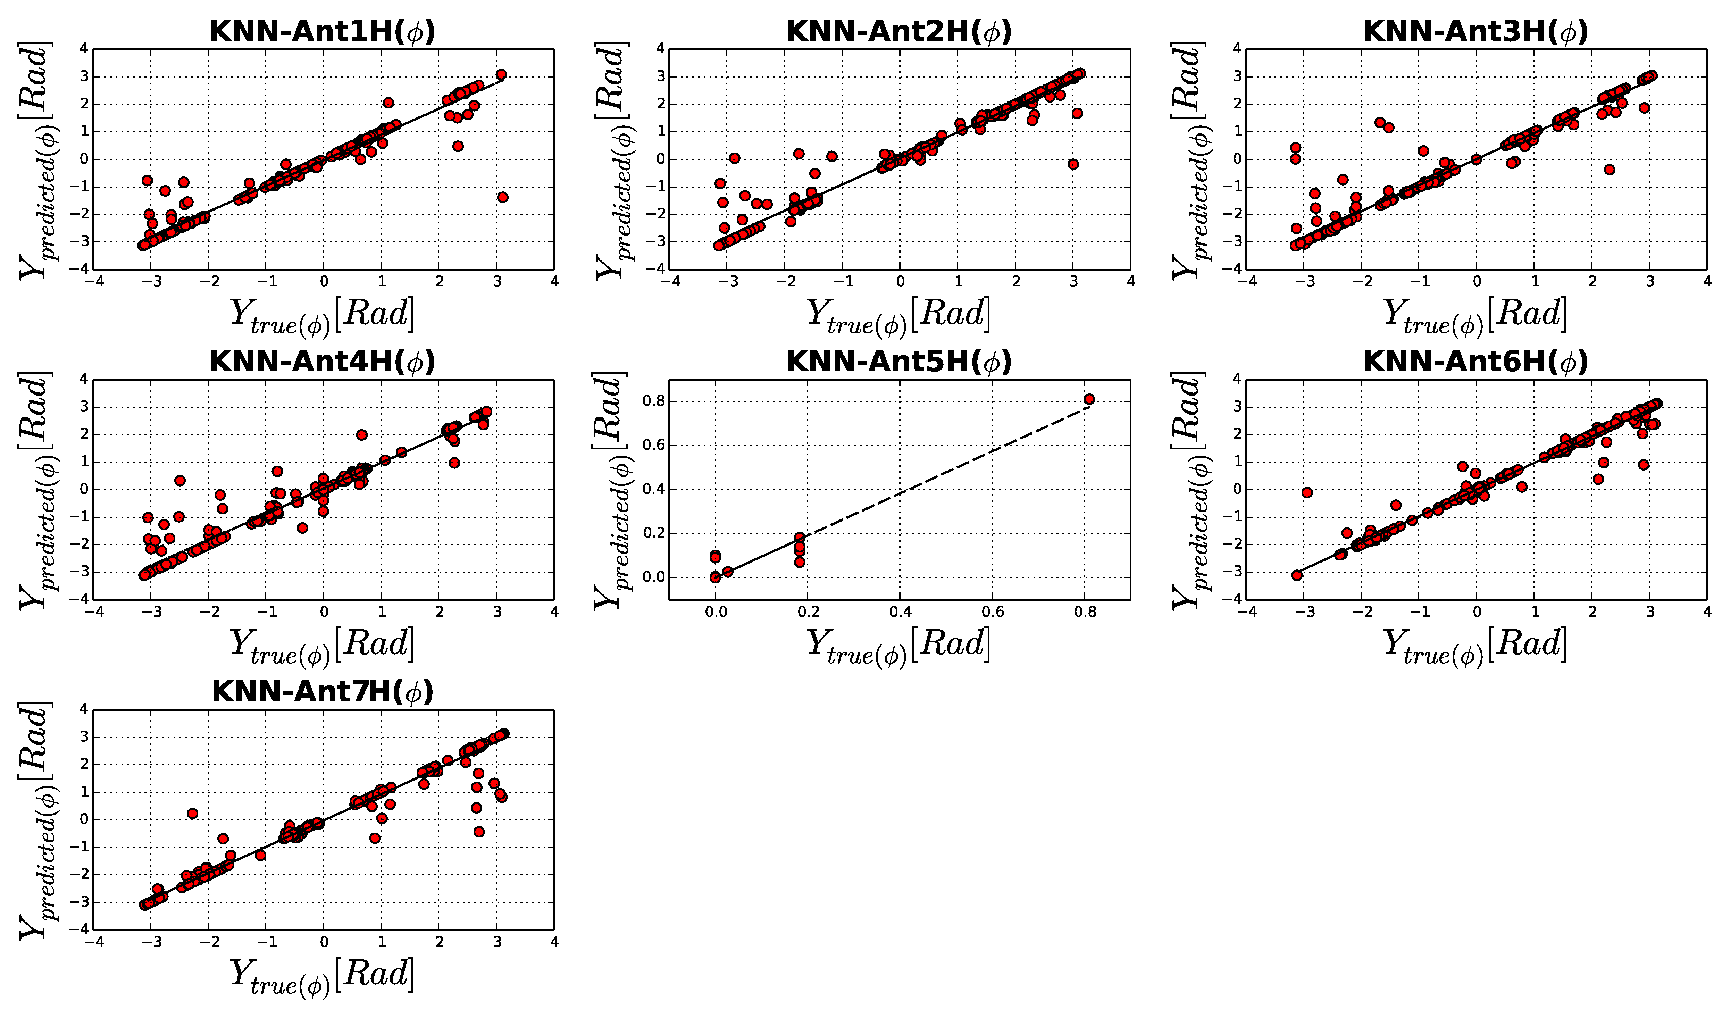
\includegraphics[width=\textwidth]{images/KNNHphase.eps} 
        \caption{Phase gain solutions for h polarization} \label{A4}
    \end{subfigure}
    
      \begin{subfigure}[t]{0.52\textheight}
       
        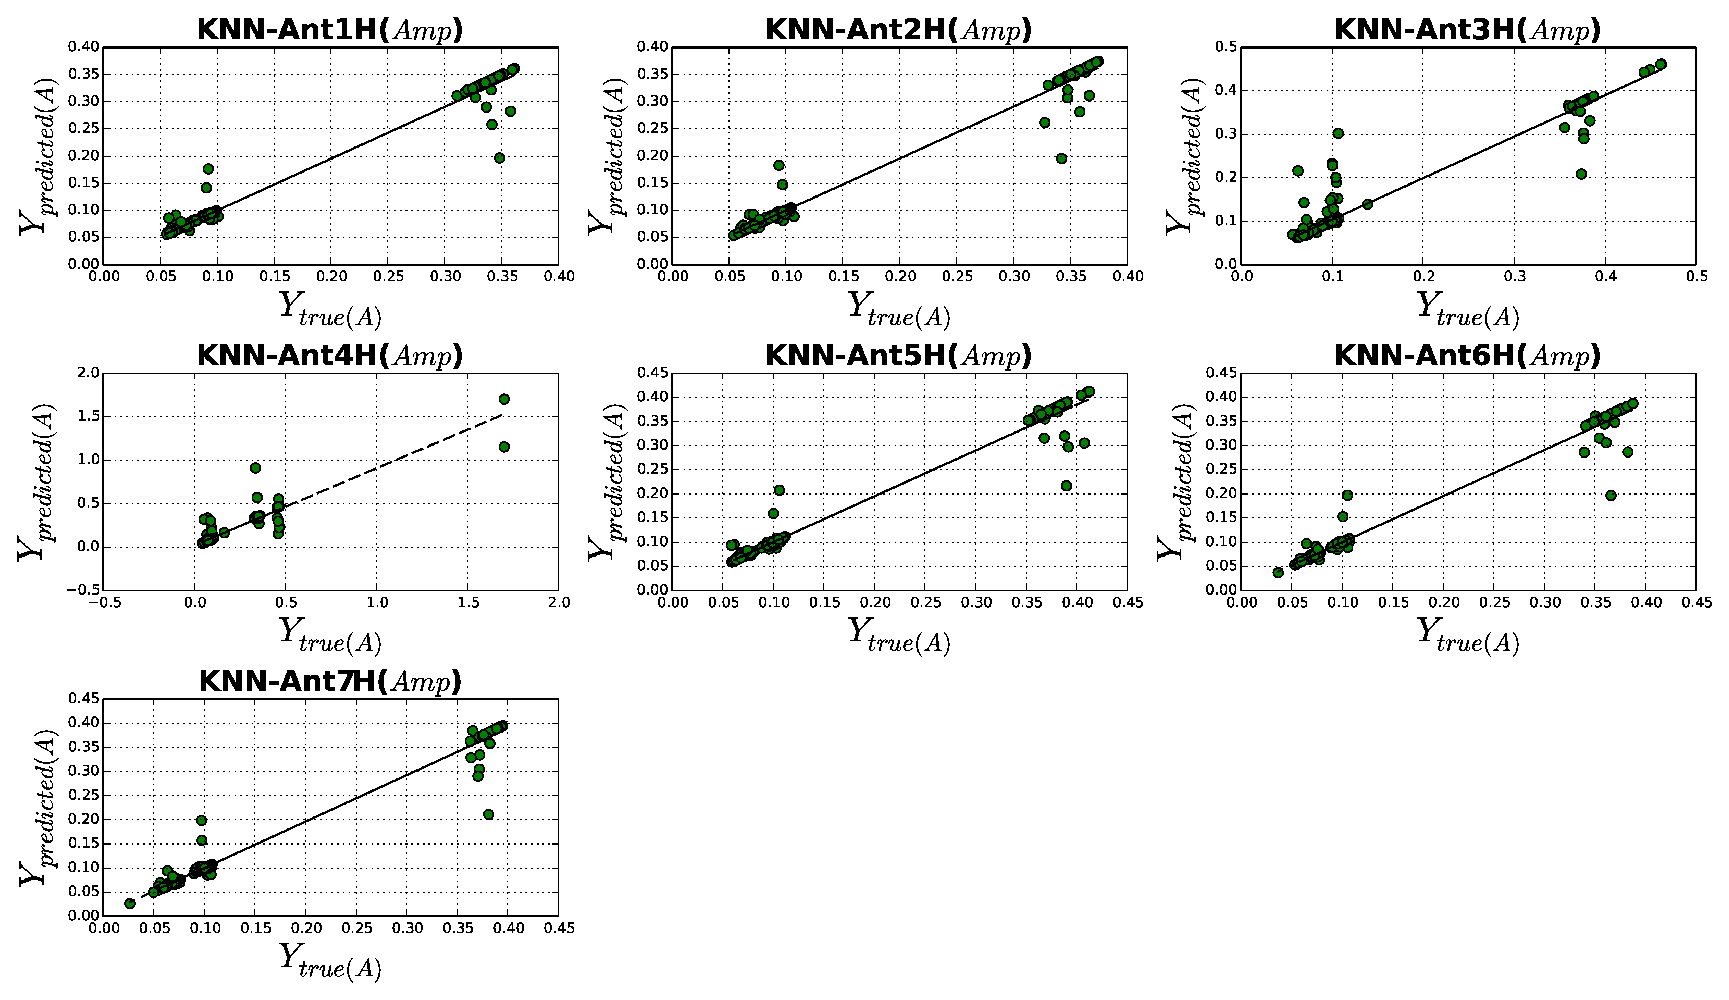
\includegraphics[width=\textwidth]{images/KNNHamp.eps} 
        \caption{Amplitude gain solutions for h polarization} \label{B4}
    \end{subfigure}
    \caption{Demonstrates the results obtained from the K-nearest neighbor learning algorithm with randomized search optimization algorithm. (\subref{A4}) and (\subref{B4}) is the predicted phase gain solutions $\textbf{Y}_{predicted}$ by the learning algorithm vs the true phase gain solutions $\textbf{Y}_{true}$ (CASA) for h polarization in radians. }
    \end{figure}
    
\begin{figure}[H]
   \centering
    \begin{subfigure}[t]{0.52\textheight}
        
        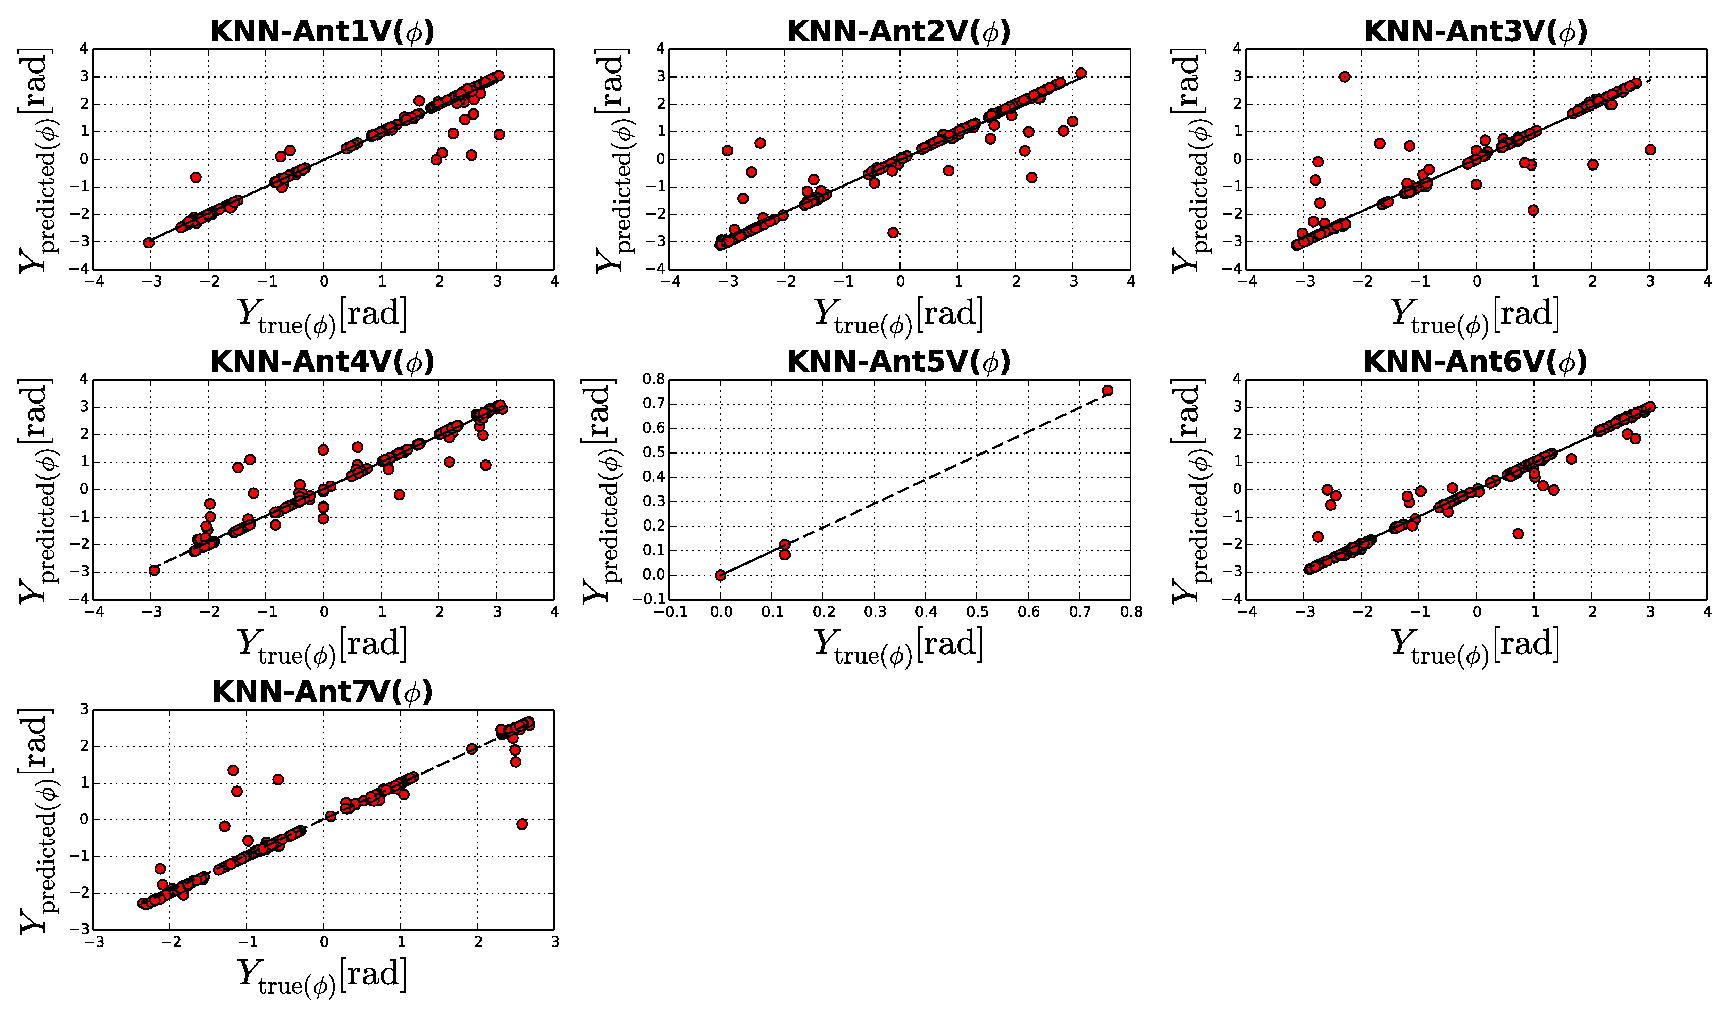
\includegraphics[width=\textwidth]{images/KNNVphase.eps} 
        \caption{Phase gain solutions for v polarization} \label{A5}
    \end{subfigure}
    
      \begin{subfigure}[t]{0.52\textheight}
       
        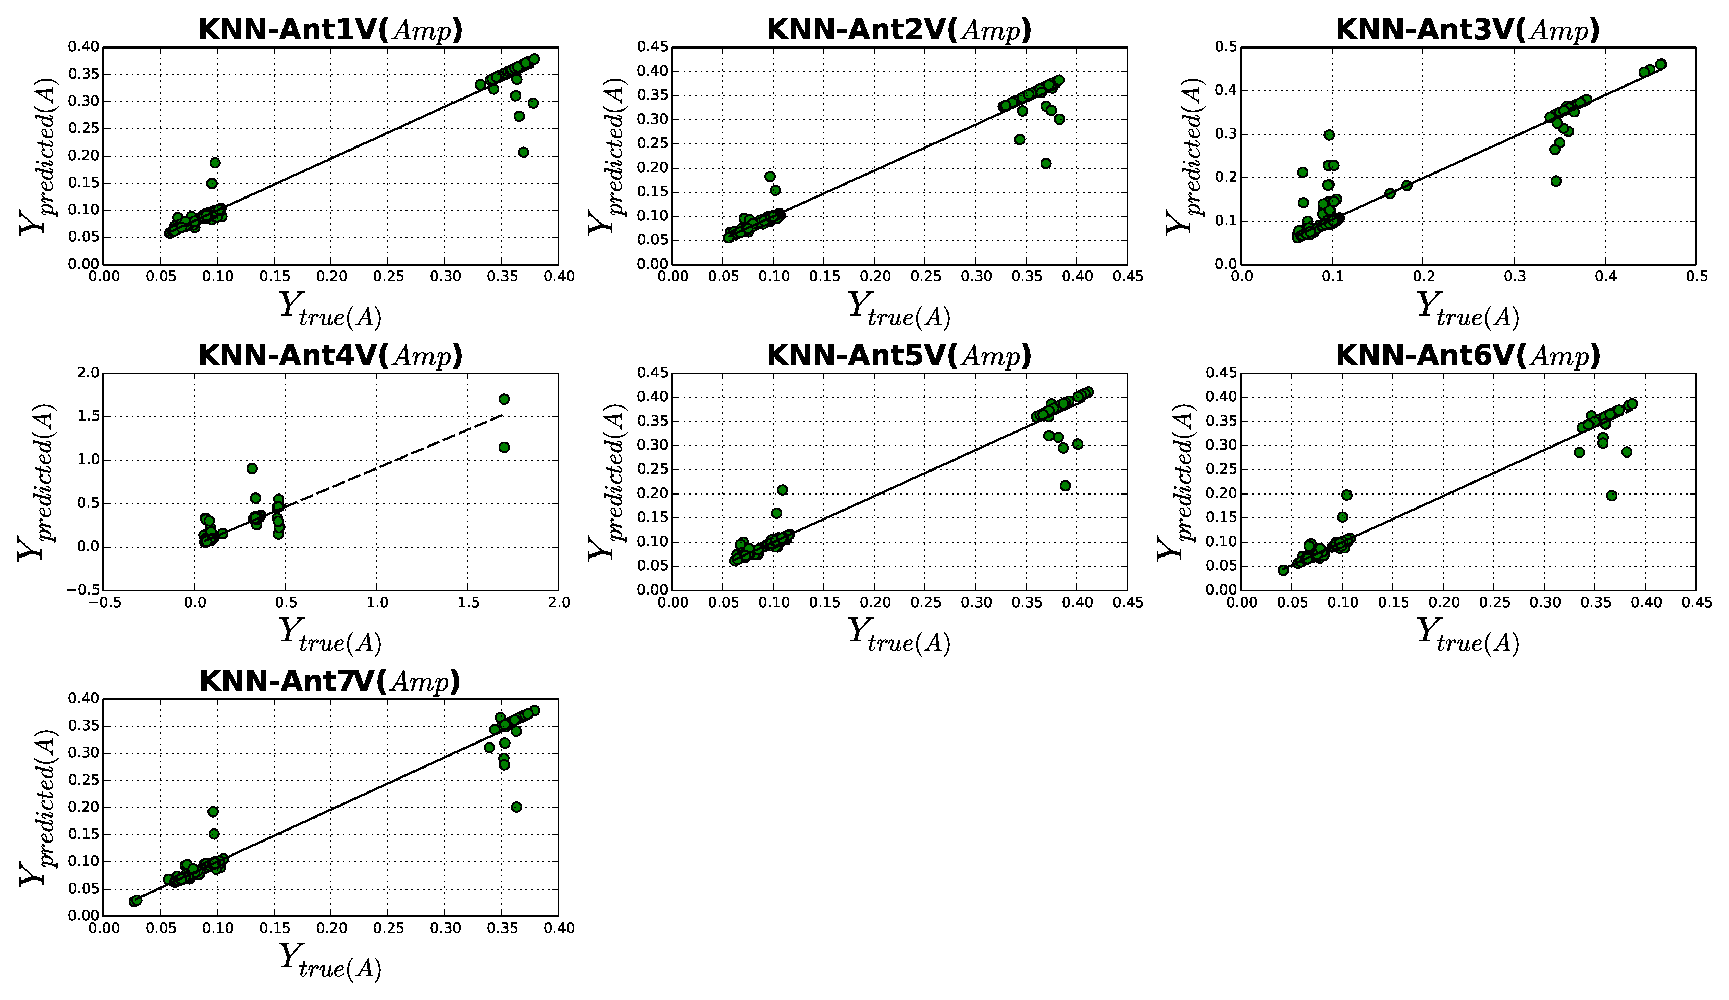
\includegraphics[width=\textwidth]{images/KNNVamp.eps} 
        \caption{Amplitude gain solutions for v polarization} \label{B5}
    \end{subfigure}
    \caption{Demonstrates the results obtained from the K-nearest neighbor learning algorithm with randomized search optimization algorithm. (\subref{A5}) and (\subref{B5}) is the predicted phase gain solutions $\textbf{Y}_{predicted}$ by the learning algorithm vs the true phase gain solutions $\textbf{Y}_{true}$ (CASA) for v polarization in radians. }
    \end{figure} 
   

\begin{table}[H]
\label{T:equipos}
\begin{center}
\scalebox{0.7}{
\begin{tabular}{| c | c | c | c | c |}
\hline
Antenna & \multicolumn{4}{ c |}{\textbf{KNN Phase}}  \\ 
\cline{2-5}
& Rmse &Rmae &R2score&Explained$\sigma^2$\\
\hline

 Uniform average-H &0.352 & 0.258 & 0.945    & 0.945 \\ 
Uniform average-V &0.291 & 0.239 & 0.961    & 0. 961\\ \hline
 & \multicolumn{4}{ c |}{\textbf{KNN Amplitude}}  \\ 
\cline{1-5}
\hline
 Uniform average-H &0.352 & 0.258 & 0.945    & 0.945 \\ 
Uniform average-V &0.291 & 0.239 & 0.961    & 0. 961\\ \hline
\end{tabular}}
\end{center}
\caption{The table shows the performance of the K-nearest neighbor algorithm in predicting the amplitude and phase gain solutions for both h and v polarizations. The values shown represents the uniform average of all KAT-7 antennas, i.e, all outputs measures are averaged with uniform weight. Majority of the predictions stay near the ideal truth values with RMSE \ref{MSE} and rmae \ref{MAE}  $\approx <$ 0.5, $R^2$ \ref{R2score} and explained variance V \ref{ExV} are converging to 1.}
\end{table}


\subsection{Extremely randomized tree-RUN}

\begin{figure}[H]
   \centering
    \begin{subfigure}[t]{0.52\textheight}
        
        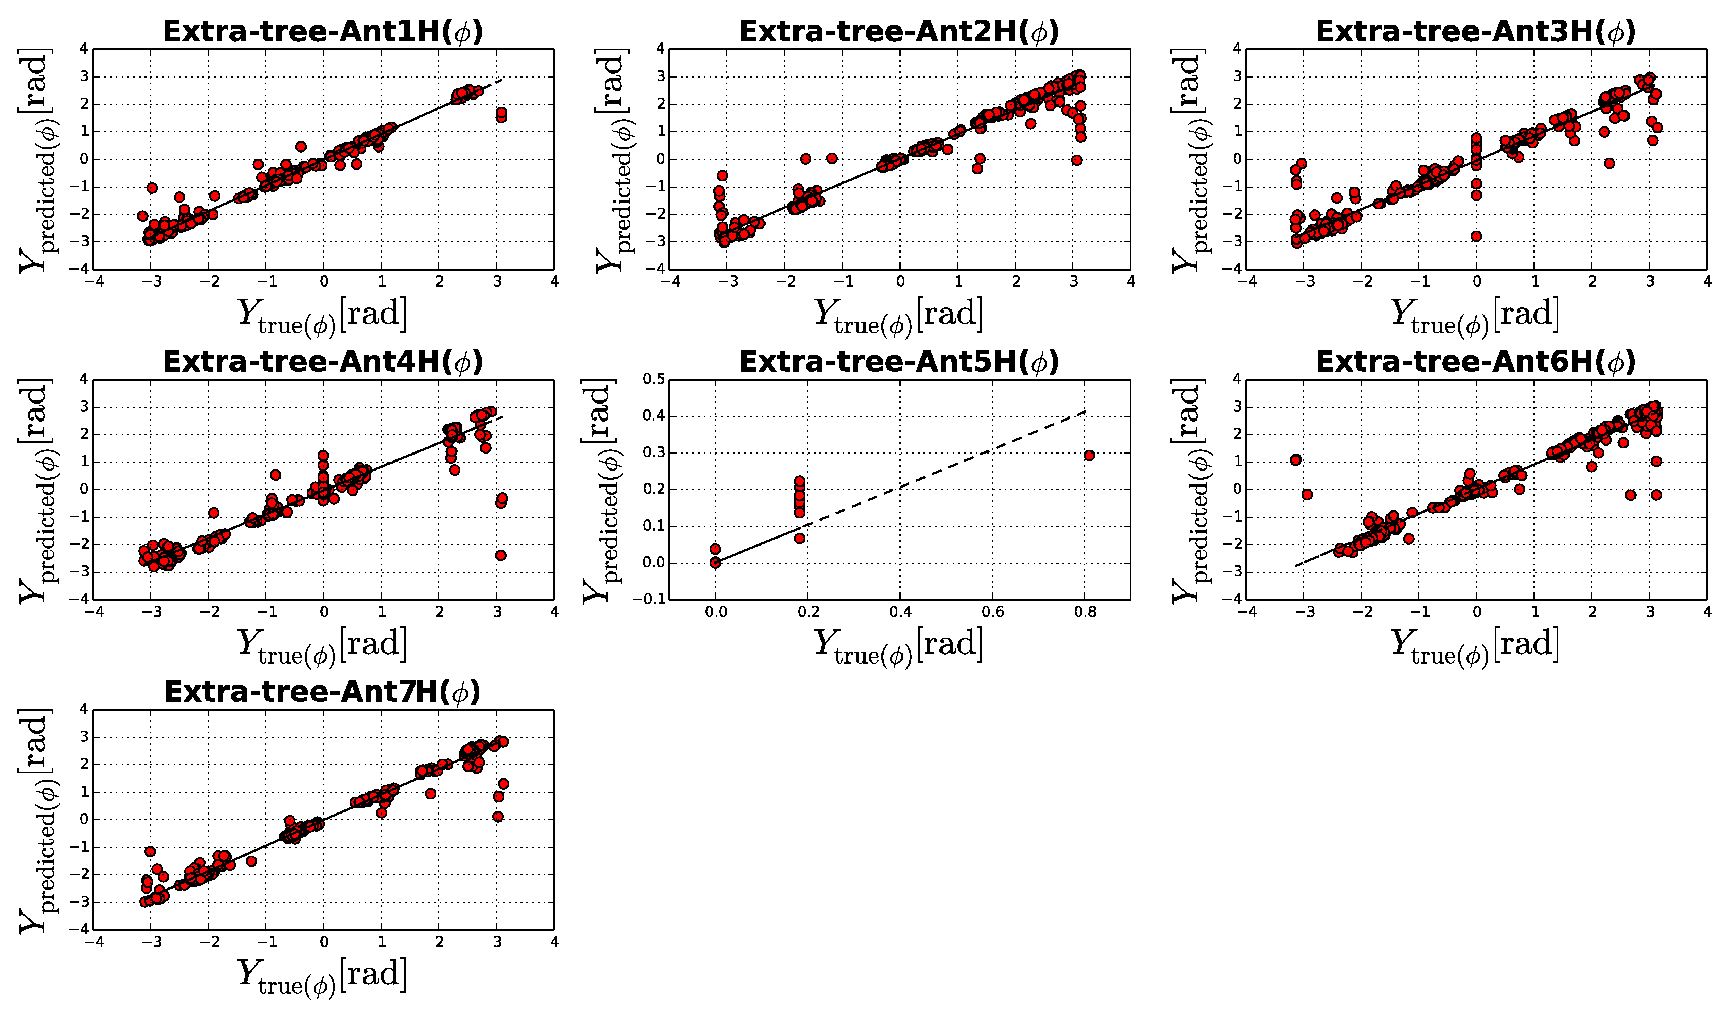
\includegraphics[width=\textwidth]{images/Extra-treeHphase.eps} 
        \caption{Phase gain solutions for h polarization} \label{A6}
    \end{subfigure}
    
      \begin{subfigure}[t]{0.52\textheight}
       
        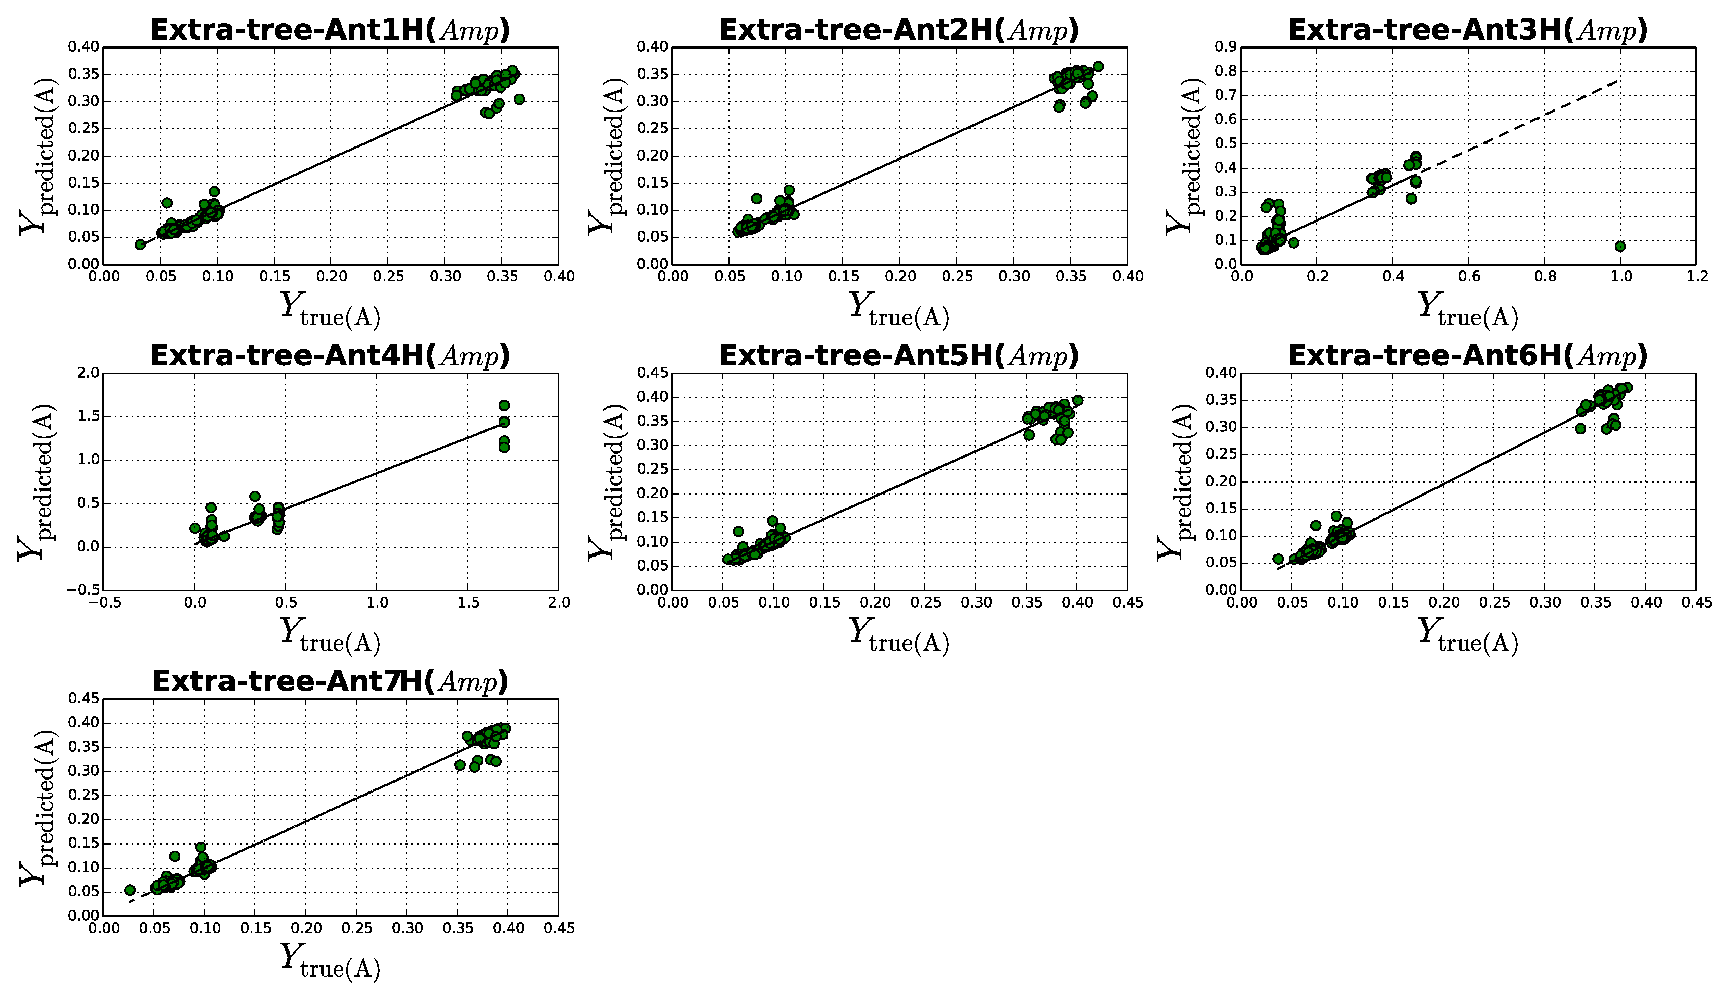
\includegraphics[width=\textwidth]{images/Extra-treeHamp.eps} 
        \caption{Amplitude gain solutions for h polarization} \label{B6}
    \end{subfigure}
    \caption{Demonstrates the results obtained from the K-nearest neighbor learning algorithm with randomized search optimization algorithm. (\subref{A6}) and (\subref{B6}) is the predicted phase gain solutions $\textbf{Y}_{predicted}$ by the learning algorithm vs the true phase gain solutions $\textbf{Y}_{true}$ (CASA) for h polarization in radians.}
    \end{figure}
    
\begin{figure}[H]
   \centering
    \begin{subfigure}[t]{0.52\textheight}
        
        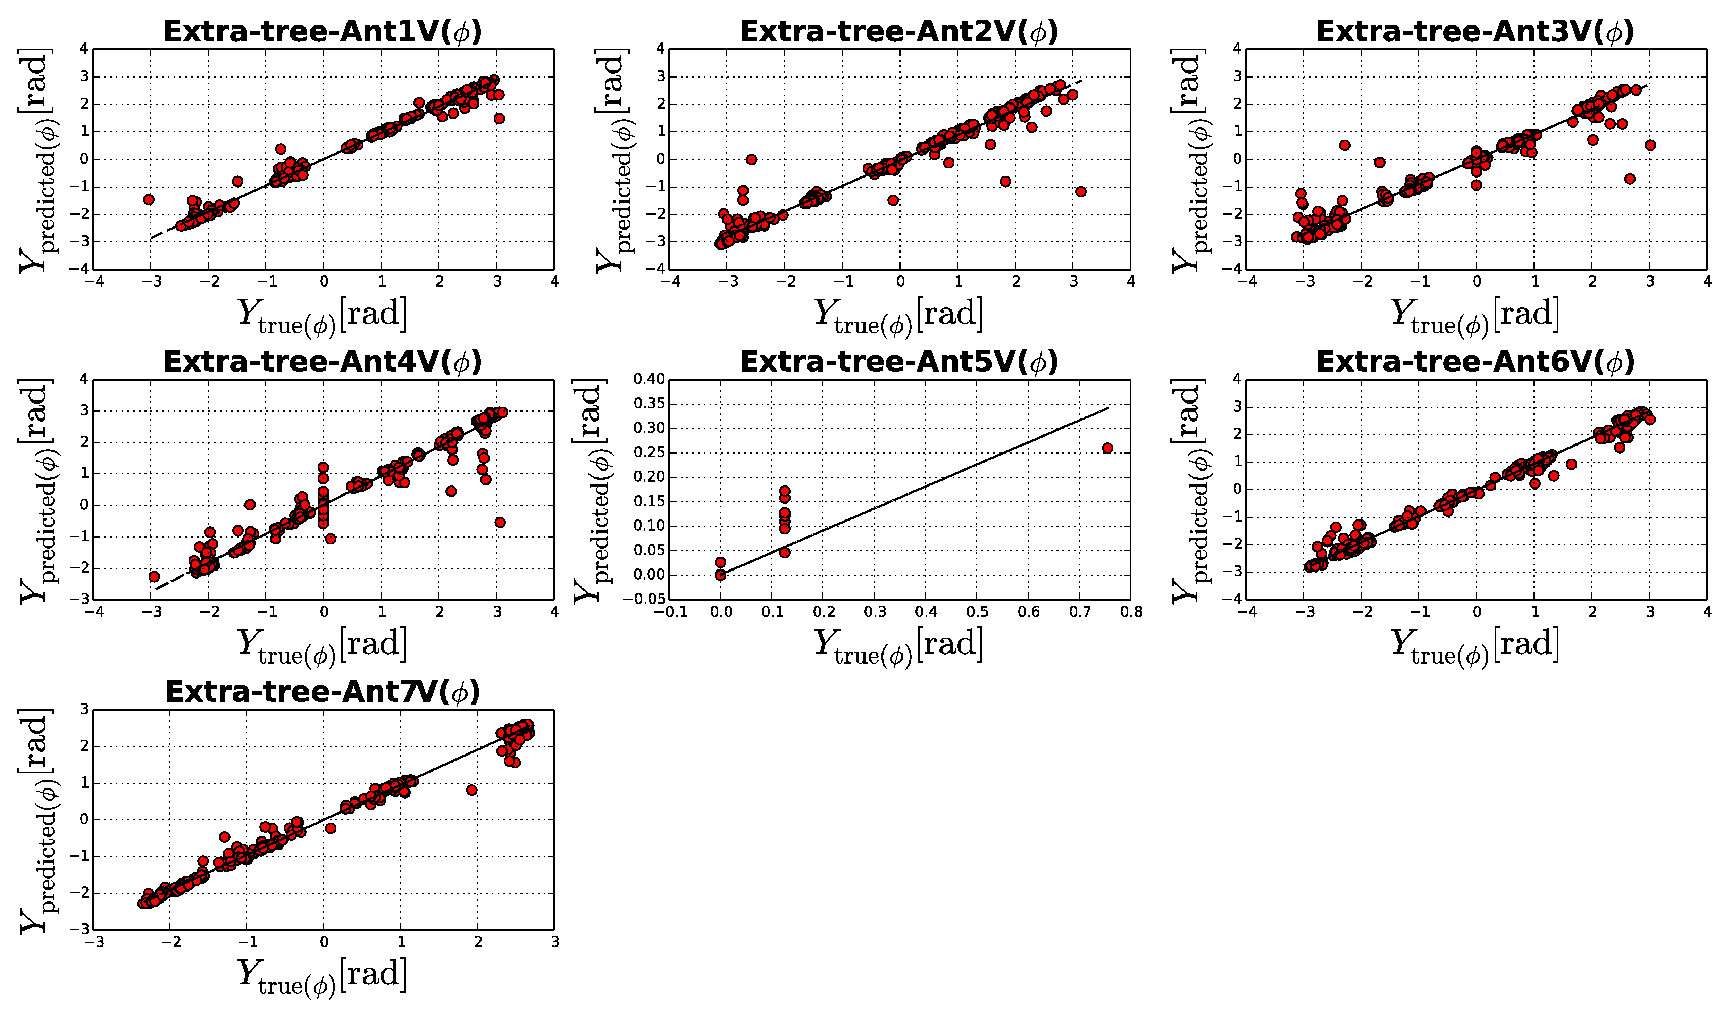
\includegraphics[width=\textwidth]{images/Extra-treeVphase.eps} 
        \caption{Phase gain solutions for v polarization} \label{A7}
    \end{subfigure}
    
      \begin{subfigure}[t]{0.52\textheight}
       
        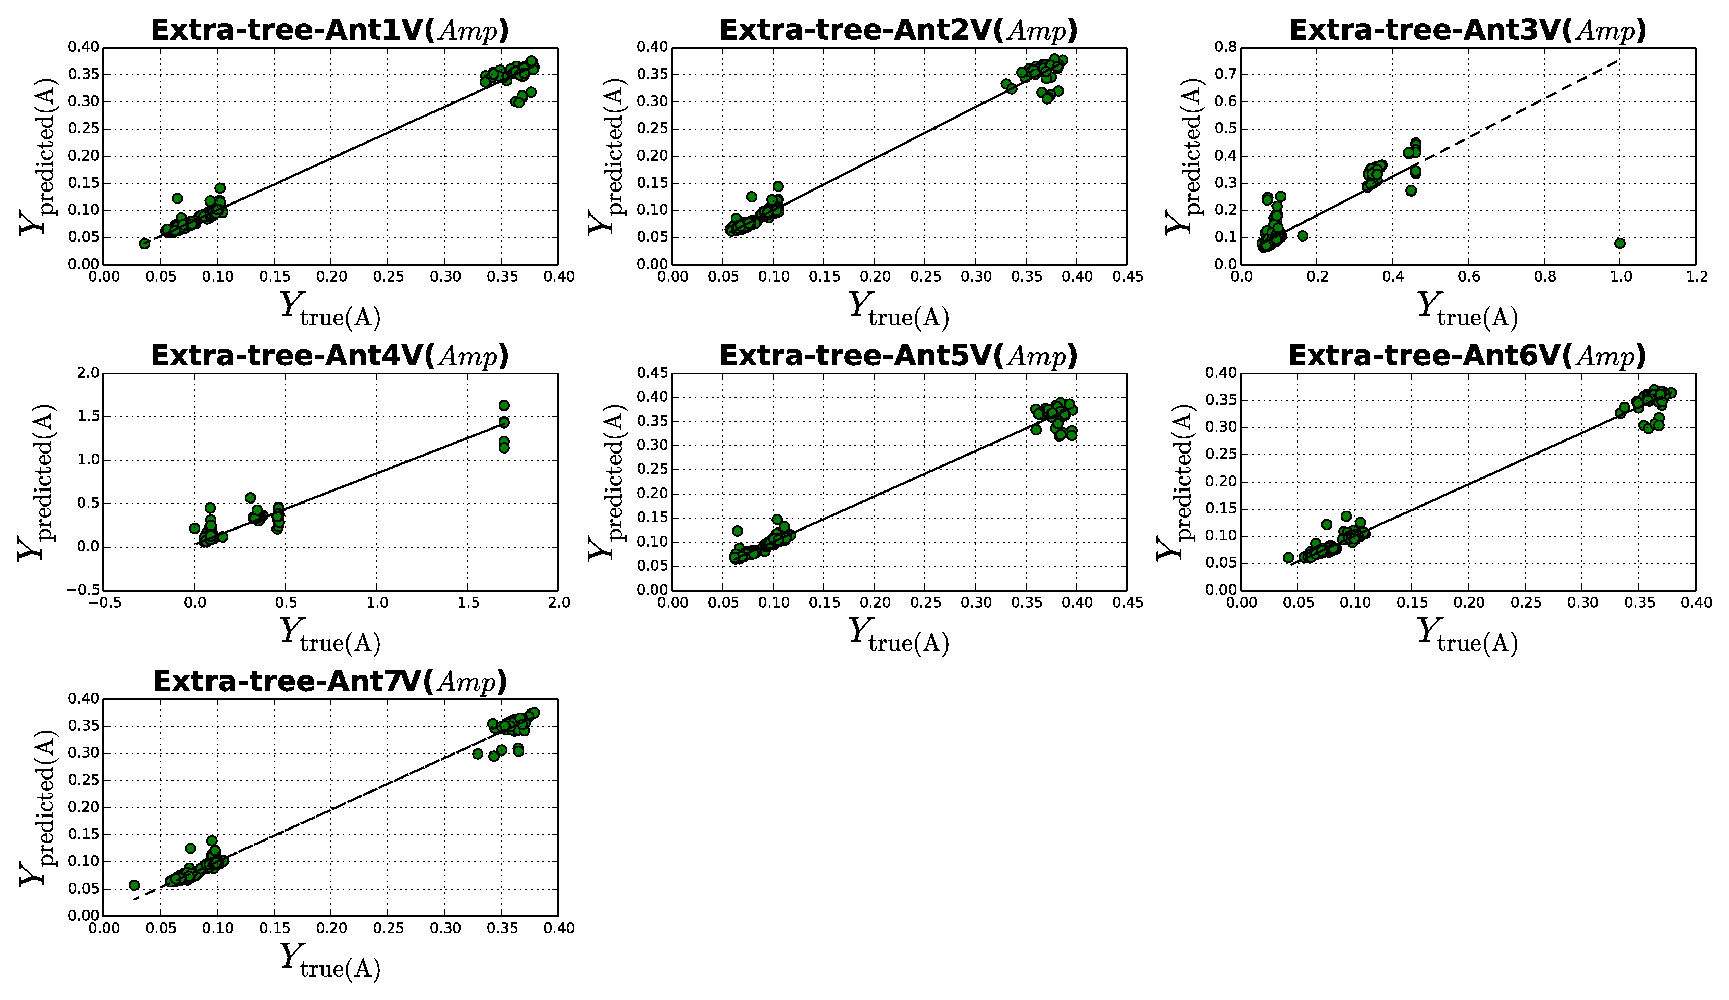
\includegraphics[width=\textwidth]{images/Extra-treeVamp.eps} 
        \caption{Amplitude gain solutions for v polarization} \label{B7}
    \end{subfigure}
    \caption{Demonstrates the results obtained from the K-nearest neighbor learning algorithm with randomized search optimization algorithm. (\subref{A7}) and (\subref{B7}) is the predicted phase gain solutions $\textbf{Y}_{predicted}$ by the learning algorithm vs the true phase gain solutions $\textbf{Y}_{true}$ (CASA) for v polarization in radians.}
    \end{figure} 
   
\begin{table}[H]
\label{T:equipos}
\begin{center}
\scalebox{0.7}{
\begin{tabular}{| c | c | c | c | c |}
\hline
Antenna & \multicolumn{4}{ c |}{\textbf{Extremely randomized Phase}}  \\ 
\cline{2-5}
& rmse & Rmae & R2score & Explained $\sigma^2$\\
\hline
 Uniform average-H &0.337 & 0.336 & 0.936    & 0.936 \\ 
Uniform average-V &0.235 & 0.301 & 0.956    & 0. 957\\ \hline
 & \multicolumn{4}{ c |}{\textbf{Extremely randomized tree  Amplitude}}  \\ 
\cline{1-5}
\hline
Uniform average-H &0.027 & 0.083 & 0.925    & 0.925 \\ 
Uniform average-V &0.027 & 0.083 & 0.923    & 0.923 \\ \hline
\end{tabular}}
\end{center}
\caption{The table shows the performance of the Extremely randomized tree algorithm in predicting the amplitude and phase gain solutions for both h and v polarizations. The values shown represents the uniform average of all KAT-7 antennas, i.e, all outputs measures are averaged with uniform weight. Majority of the predictions stay near the ideal truth values with rmse \ref{MSE} and rmae \ref{MAE}  $\approx <$ 0.5, $R^2$ \ref{R2score} and explained variance V \ref{ExV} are converging to 1.}
\end{table}

 %When fitting a straight line(slope) between the predicted and the true we  observe there is only few outlying points.
\subsection{Testing on new dataset}

Now that we are happy with the performance of our learning algorithms in predicting the calibration solutions accurately from the testing dataset. In this section we use new sensor data extracted from new(unseen) KAT-7 observations with the phase calibrator source PKS1623-586 to predict the calibration solutions. This process is called model validation. Since our model was trained on normalized data, we first normalize the new sensor data with mean $\mu$ and standard deviation $\sigma$ obtained from the normalization of the training dataset.
\begin{align}
\text{scaled-sensor data}= \frac{\text{sensor data}- \mu}{\sigma}
\end{align}

\subsubsection{Observation test-1}
In this section, we show plot results obtained from the validation dataset-1. 
 \begin{figure}[H]
    \includegraphics[ height=13cm, width=16cm]{images/Phasegain.eps}
    \caption{This figure is showing the response of the decision tree learning algorithm in predicting the phase gain solutions for the calibrator PKS1613-586 from the validation dataset-1. In each subplot we show the CASA calculated phase gain solutions for h (blue) and v (green) polarization vs the learning algorithm (ZCal) predicted phase gain solutions for h (red) and v (yellow) polarization.}
    \label{obs1}
\end{figure}

\begin{figure}[H]
    \includegraphics[ height=13cm, width=16cm]{images/DCampgain.eps}
    \caption{This figure is showing the response of the decision tree learning algorithm in predicting the amplitude gain solutions for the calibrator PKS1613-586 from the validation dataset-1. In each subplot we show the CASA calculated amplitude gain solutions for h (blue) and v (green) polarization vs the learning algorithm (ZCal) predicted amplitude gain solutions for h (red) and v (yellow) polarization.}
     \label{da1}
\end{figure}


\begin{figure}[H]
    \includegraphics[ height=13cm, width=16cm]{images/RFphasegain.eps}
    \caption{This figure is showing the response of the random forest learning algorithm in predicting the phase gain solutions for the calibrator PKS1613-586 from the validation dataset-1. In each subplot we show the CASA calculated phase gain solutions for h (blue) and v (green) polarization vs the learning algorithm (ZCal) predicted phase gain solutions for h (red) and v (yellow) polarization.}
    \label{obs2}
\end{figure}

\begin{figure}[H]
    \includegraphics[ height=13cm, width=16cm]{images/RFampegain.eps}
    \caption{This figure is showing the response of the random forest learning algorithm in predicting the amplitude gain solutions for the calibrator PKS1613-586 from the validation dataset-1. In each subplot we show the CASA calculated amplitude gain solutions for h (blue) and v (green) polarization vs the learning algorithm (ZCal) predicted amplitude gain solutions for h (red) and v (yellow) polarization.}
     \label{ra1}
\end{figure}


\begin{figure}[H]
    \includegraphics[ height=13cm, width=16cm]{images/KNNPhasegain.eps}
    \caption{This figure is showing the response of the K-nearest neighbor learning algorithm in predicting the phase gain solutions for the calibrator PKS1613-586 from the validation dataset-1. In each subplot we show the CASA calculated phase gain solutions for h (blue) and v (green) polarization vs the learning algorithm (ZCal) predicted phase gain solutions for h (red) and v (yellow) polarization.}
    \label{obs3}
\end{figure}

\begin{figure}[H]
    \includegraphics[ height=13cm, width=16cm]{images/KNNampgain.eps}
    \caption{This figure is showing the response of the K-nearest neighbor learning algorithm in predicting the amplitude gain solutions for the calibrator PKS1613-586 from the validation dataset-1. In each subplot we show the CASA calculated amplitude gain solutions for h (blue) and v (green) polarization vs the learning algorithm (ZCal) predicted amplitude gain solutions for h (red) and v (yellow) polarization.}
     \label{ka1}
\end{figure}

\begin{figure}[H]
    \includegraphics[ height=13cm, width=16cm]{images/EXTPhasegain.eps}
    \caption{This figure is showing the response of the extremely randomized tree learning algorithm in predicting the phase gain solutions for the calibrator PKS1613-586 from the validation dataset-1. In each subplot we show the CASA calculated phase gain solutions for h (blue) and v (green) polarization vs the learning algorithm (ZCal) predicted phase gain solutions for h (red) and v (yellow) polarization.}
    \label{obs4}
\end{figure}

\begin{figure}[H]
    \includegraphics[ height=13cm, width=16cm]{images/EXTampgain.eps}
    \caption{This figure is showing the response of the extremely randomized tree learning algorithm in predicting the amplitude gain solutions for the calibrator PKS1613-586 from the validation dataset-1. In each subplot we show the CASA calculated amplitude gain solutions for h (blue) and v (green) polarization vs the learning algorithm (ZCal) predicted amplitude gain solutions for h (red) and v (yellow) polarization.}
     \label{ea1}
\end{figure}

\subsubsection{Observation test-2}
In this section, we show plot results obtained from the validation dataset-2. 
\begin{figure}[H]
    \includegraphics[ height=13cm, width=16cm]{images/DCPhasegain1015.eps}
    \caption{This figure is showing the response of the decision tree learning algorithm in predicting the phase gain solutions for the calibrator PKS1613-586 from the validation dataset-2. In each subplot we show the CASA calculated phase gain solutions for h (blue) and v (green) polarization vs the learning algorithm (ZCal) predicted phase gain solutions for h (red) and v (yellow) polarization.}
    \label{obs5}
\end{figure}

\begin{figure}[H]
    \includegraphics[ height=13cm, width=16cm]{images/DCampgain1015.eps}
    \caption{This figure is showing the response of the decision tree learning algorithm in predicting the amplitude gain solutions for the calibrator PKS1613-586 from the validation dataset-2. In each subplot we show the CASA calculated amplitude gain solutions for h (blue) and v (green) polarization vs the learning algorithm (ZCal) predicted amplitude gain solutions for h (red) and v (yellow) polarization.}
     \label{da2}
\end{figure}


\begin{figure}[H]
    \includegraphics[ height=13cm, width=16cm]{images/RFPhasegain1015.eps}
    \caption{This figure is showing the response of the random forest learning algorithm in predicting the phase gain solutions for the calibrator PKS1613-586 from the validation dataset-2. In each subplot we show the CASA calculated phase gain solutions for h (blue) and v (green) polarization vs the learning algorithm (ZCal) predicted phase gain solutions for h (red) and v (yellow) polarization.}
    \label{obs6}
\end{figure}

\begin{figure}[H]
    \includegraphics[ height=13cm, width=16cm]{images/RFampgain1015.eps}
    \caption{This figure is showing the response of the random forest learning algorithm in predicting the amplitude gain solutions for the calibrator PKS1613-586 from the validation dataset-2. In each subplot we show the CASA calculated amplitude gain solutions for h (blue) and v (green) polarization vs the learning algorithm (ZCal) predicted amplitude gain solutions for h (red) and v (yellow) polarization.}
     \label{ra2}
\end{figure}

\begin{figure}[H]
    \includegraphics[ height=13cm, width=16cm]{images/KNNPhasegain1015.eps}
    \caption{This figure is showing the response of the K-nearest neighbor learning algorithm in predicting the phase gain solutions for the calibrator PKS1613-586 from the validation dataset-2. In each subplot we show the CASA calculated phase gain solutions for h (blue) and v (green) polarization vs the learning algorithm (ZCal) predicted phase gain solutions for h (red) and v (yellow) polarization.}
    \label{obs7}
\end{figure}

\begin{figure}[H]
    \includegraphics[ height=13cm, width=16cm]{images/KNNampgain1015.eps}
    \caption{This figure is showing the response of the K-nearest neighbor learning algorithm in predicting the amplitude gain solutions for the calibrator PKS1613-586 from the validation dataset-2. In each subplot we show the CASA calculated amplitude gain solutions for h (blue) and v (green) polarization vs the learning algorithm (ZCal) predicted amplitude gain solutions for h (red) and v (yellow) polarization.}
     \label{ka2}
\end{figure}

\begin{figure}[H]
    \includegraphics[ height=13cm, width=16cm]{images/EXTPhasegain1015.eps}
    \caption{This figure is showing the response of the extremely randomized tree learning algorithm in predicting the phase gain solutions for the calibrator PKS1613-586 from the validation dataset-2. In each subplot we show the CASA calculated phase gain solutions for h (blue) and v (green) polarization vs the learning algorithm (ZCal) predicted phase gain solutions for h (red) and v (yellow) polarization.}
    \label{obs8}
\end{figure}

\begin{figure}[H]
    \includegraphics[ height=13cm, width=16cm]{images/EXTampgain1015.eps}
    \caption{This figure is showing the response of the extremely randomized tree learning algorithm in predicting the amplitude gain solutions for the calibrator PKS1613-586 from the validation dataset-2. In each subplot we show the CASA calculated amplitude gain solutions for h (blue) and v (green) polarization vs the learning algorithm (ZCal) predicted amplitude gain solutions for h (red) and v (yellow) polarization.}
     \label{ea2}
\end{figure}


\subsubsection{Observation test-3}
In this section, we show plot results obtained from the validation dataset-3. 
\begin{figure}[H]
    \includegraphics[ height=13cm, width=16cm]{images/DCPhasegain773.eps}
    \caption{This figure is showing the response of the decision tree learning algorithm in predicting the phase gain solutions for the calibrator PKS1613-586 from the validation dataset-3. In each subplot we show the CASA calculated phase gain solutions for h (blue) and v (green) polarization vs the learning algorithm (ZCal) predicted phase gain solutions for h (red) and v (yellow) polarization.}
    \label{obs9}
\end{figure}

\begin{figure}[H]
    \includegraphics[ height=13cm, width=16cm]{images/DCampgain773.eps}
    \caption{This figure is showing the response of the decision tree learning algorithm in predicting the amplitude gain solutions for the calibrator PKS1613-586 from the validation dataset-3. In each subplot we show the CASA calculated amplitude gain solutions for h (blue) and v (green) polarization vs the learning algorithm (ZCal) predicted amplitude gain solutions for h (red) and v (yellow) polarization.}
     \label{da3}
\end{figure}


\begin{figure}[H]
    \includegraphics[ height=13cm, width=16cm]{images/RFPhasegain773.eps}
    \caption{This figure is showing the response of the random forest learning algorithm in predicting the phase gain solutions for the calibrator PKS1613-586 from the validation dataset-3. In each subplot we show the CASA calculated phase gain solutions for h (blue) and v (green) polarization vs the learning algorithm (ZCal) predicted phase gain solutions for h (red) and v (yellow) polarization.}
    \label{obs10}
\end{figure}

\begin{figure}[H]
    \includegraphics[ height=13cm, width=16cm]{images/RFampgain773.eps}
    \caption{This figure is showing the response of the random forest learning algorithm in predicting the amplitude gain solutions for the calibrator PKS1613-586 from the validation dataset-3. In each subplot we show the CASA calculated amplitude gain solutions for h (blue) and v (green) polarization vs the learning algorithm (ZCal) predicted amplitude gain solutions for h (red) and v (yellow) polarization.}
     \label{ra3}
\end{figure}

\begin{figure}[H]
    \includegraphics[ height=13cm, width=16cm]{images/KNNPhasegain773.eps}
    \caption{This figure is showing the response of the K-nearest neighbor learning algorithm in predicting the phase gain solutions for the calibrator PKS1613-586 from the validation dataset-3. In each subplot we show the CASA calculated phase gain solutions for h (blue) and v (green) polarization vs the learning algorithm (ZCal) predicted phase gain solutions for h (red) and v (yellow) polarization.}
    \label{obs11}
\end{figure}

\begin{figure}[H]
    \includegraphics[ height=13cm, width=16cm]{images/KNNampgain773.eps}
    \caption{This figure is showing the response of the K-nearest neighbor learning algorithm in predicting the amplitude gain solutions for the calibrator PKS1613-586 from the validation dataset-3. In each subplot we show the CASA calculated amplitude gain solutions for h (blue) and v (green) polarization vs the learning algorithm (ZCal) predicted amplitude gain solutions for h (red) and v (yellow) polarization.}
     \label{ka3}
\end{figure}

\begin{figure}[H]
    \includegraphics[ height=13cm, width=16cm]{images/EXTPhasegain773.eps}
    \caption{This figure is showing the response of the extremely randomized tree learning algorithm in predicting the phase gain solutions for the calibrator PKS1613-586 from the validation dataset-3. In each subplot we show the CASA calculated phase gain solutions for h (blue) and v (green) polarization vs the learning algorithm (ZCal) predicted phase gain solutions for h (red) and v (yellow) polarization.}
    \label{obs12}
\end{figure}

\begin{figure}[H]
    \includegraphics[ height=13cm, width=16cm]{images/EXTampgain773.eps}
    \caption{This figure is showing the response of the extremely randomized tree learning algorithm in predicting the amplitude gain solutions for the calibrator PKS1613-586 from the validation dataset-3. In each subplot we show the CASA calculated amplitude gain solutions for h (blue) and v (green) polarization vs the learning algorithm (ZCal) predicted amplitude gain solutions for h (red) and v (yellow) polarization.}
     \label{ea3}
\end{figure}













